%% Effect Identity for LLM Agents: Schema-Determined Limits on Duplicate Suppression
%% Manuscript for Artificial Intelligence (Elsevier), ISSN 0004-3702.
%%
%% Build (figure data from results/ -> number checks -> pdflatex/bibtex):
%%   node docs/research/aij/build.mjs
%% Every interval of the form NN.N\%~[lo--hi] in this manuscript is checked
%% against research/effect-identity/results/*.json by the build; see
%% research/effect-identity/src/experiments/checkPaper.js.
\documentclass[preprint,review,12pt]{elsarticle}

\usepackage[T1]{fontenc}
\usepackage[utf8]{inputenc}
\usepackage{lmodern}
\usepackage{amsmath,amssymb}
\usepackage{stmaryrd}
\usepackage{amsthm}
\usepackage{longtable}
\usepackage{booktabs,array,tabularx}
\usepackage{graphicx}
\usepackage{xcolor}
\usepackage{tikz}
\usetikzlibrary{arrows.meta,positioning,fit,calc,shapes.geometric,backgrounds,patterns}
\usepackage{pgfplots}
\pgfplotsset{compat=1.16}
\usepackage[ruled,vlined,linesnumbered]{algorithm2e}
\usepackage[shortlabels]{enumitem}
\usepackage{url}
\usepackage{hyperref}
\hypersetup{colorlinks=true,linkcolor=blue!50!black,citecolor=blue!50!black,urlcolor=blue!50!black}
\usepackage{lineno}

\newtheorem{theorem}{Theorem}
\newtheorem{proposition}{Proposition}
\newtheorem{lemma}{Lemma}
\newtheorem{corollary}{Corollary}
\theoremstyle{definition}
\newtheorem{definition}{Definition}
\theoremstyle{remark}
\newtheorem{remark}{Remark}

\newcommand{\WS}{\mathrm{WS}}
\newcommand{\Res}{\mathrm{Res}}
\newcommand{\Dec}{\mathrm{Dec}}
\newcommand{\thi}{t_{\mathrm{hi}}}
\newcommand{\tlo}{t_{\mathrm{lo}}}
\newcommand{\SUP}{\textsc{suppress}}
\newcommand{\EXE}{\textsc{execute}}
\newcommand{\ESC}{\textsc{escalate}}
\newcommand{\iv}[3]{#1\%~[#2--#3]}

%% Float placement: the double-spaced review layout starves the default float
%% areas, which pushes every float to the end of the document. These values let
%% a float occupy most of a page so that it lands near the text that cites it.
\renewcommand{\topfraction}{0.92}
\renewcommand{\bottomfraction}{0.75}
\renewcommand{\textfraction}{0.06}
\renewcommand{\floatpagefraction}{0.65}
\setcounter{topnumber}{3}
\setcounter{bottomnumber}{2}
\setcounter{totalnumber}{5}

\journal{Artificial Intelligence}

\begin{document}

\begin{frontmatter}
\title{Effect Identity for LLM Agents:\\ Schema-Determined Limits on Duplicate Suppression}

\author[aff1]{Sivaguru R.~M.\corref{cor1}}
\ead{sivagurumurugan1@gmail.com}
\cortext[cor1]{Corresponding author.}
\affiliation[aff1]{organization={Independent Research, AgentRuntime Project},
            city={Chennai},
            state={Tamil Nadu},
            country={India}}

\begin{abstract}
An autonomous agent that retries an irreversible action re-synthesises its arguments, so two requests for the same real-world act may share no surface token. Content-addressed keys then miss the duplicate, and an unconstrained language-model judgement offers no bound on the opposite, silent error of suppressing a distinct act. We treat effect identity as a decision under asymmetric loss with a stochastic oracle and adversarial input. Any identity procedure decomposes into a certifier that proves sameness, a refuter that proves difference, and a residual that neither settles, determined by the declared tool schema. Our fence consults an LLM judge only on the residual and suppresses only when the maximum score over the $m$ surviving candidates exceeds a conformal threshold at level $\alpha/m$. Under exchangeability, wrong suppression is bounded by $\alpha$, provided the calibration pool is drawn from the rule's own jurisdiction; a mismatched pool hides its own violation. Refining the schema or demanding class validity shrinks the calibration budget: a refinement dilemma we state exactly. On the evaluation corpus of 1,066 pairs over six tools, the fence deduplicates 94.7\% of paraphrased duplicates at 1.7\% wrong suppression, against 12.1\% for canonical keys; wrong suppression stays below $\alpha=0.05$ across three judges while deduplication ranges from 82.6\% to 94.7\%. Under seed-level resplitting, mean wrong suppression is 2.7\% with 10.5\% of splits exceeding $\alpha$. Typed fields eliminate field injection; prose-only injection succeeds 84\% of the time. Label reproducibility is audited via a blinded model panel, with contested strata evaluated through a targeted human follow-up. The mechanism provides bounded identity recognition and fence-level commitment, not external exactly-once execution.

\end{abstract}

%% Keep in sync with highlights.txt, the copy uploaded as a separate file.
\begin{highlights}
\item Effect identity for LLM agents is treated as a decision under asymmetric loss.
\item Certifier and refuter settle what the schema pins; only the residual is judged.
\item A conformal bound holds for the max-over-candidates statistic the fence uses.
\item Refining the schema shrinks the calibration pool: an exact refinement dilemma.
\item Canonical keys dedupe 12.1\%; the fence 94.7\% at 1.7\% wrong suppression.
\end{highlights}

\begin{keyword}
effect identity \sep duplicate suppression \sep LLM agents \sep conformal prediction \sep multiple comparisons \sep prompt injection \sep idempotency
\end{keyword}
\end{frontmatter}

\linenumbers
\sloppy

\section{Introduction}\label{sec:intro}

Language-model agents now routinely act through tools whose effects cannot be undone---charging cards, moving money, sending messages, creating records~\cite{yao2023react,schick2023toolformer,yao2024taubench}. When such an agent crashes, times out, or is re-prompted after a failure, its recovery path re-issues work, and the surrounding system must not perform the same irreversible action twice. The classical defence is straightforward: give each effect an identity, record it when the effect commits, and refuse a second commit under the same identity~\cite{birrell1984rpc,kleppmann2017ddia,stripe2026idempotency}. Every mechanism of this kind---journal positions in durable-execution engines~\cite{temporal2026docs,restate2026docs}, client-chosen idempotency keys~\cite{stripe2026idempotency}, hashes of a canonicalised request---answers one question implicitly: \emph{when do two requests denote the same act?}

For a deterministic program the answer is positional or syntactic, because a retried call replays the original byte for byte. An LLM agent breaks both assumptions. Its control flow is sampled, so ``the third tool call'' is not stable across retries; and more fundamentally, its \emph{arguments} are re-synthesised. An agent asked to wire \$780 to Marlow Freight for shipment 88213 may first emit
\begin{quote}\small\ttfamily
wire\_money\{\\
\hspace*{1.5em}amount\_text: "\$780.00",\\
\hspace*{1.5em}beneficiary\_text: "Marlow Freight",\\
\hspace*{1.5em}reference: "Shipment 88213"\}
\end{quote}
and, after a crash and a re-prompt, emit
\begin{quote}\small\ttfamily
wire\_money\{\\
\hspace*{1.5em}amount\_text: "seven hundred eighty dollars",\\
\hspace*{1.5em}beneficiary\_text: "MARLOW FREIGHT",\\
\hspace*{1.5em}reference: "shipment \#88213"\}
\end{quote}
The two requests canonicalise differently and hash differently, and a content-addressed fence wires the money a second time. The converse situation is equally real: two requests that differ in a single token of free text (``instalment 1 of 2'' versus ``instalment 2 of 2'') can be two legitimate acts that must both execute.

Deciding identity therefore requires interpreting arguments, and the two errors are sharply asymmetric. Executing a duplicate is costly but \emph{observable}: two committed records exist for reconciliation to find. Suppressing a distinct act is \emph{silent}: the fence returns the recorded response of an earlier act, the agent believes the new act happened, and no trace shows otherwise. We call this second error \emph{wrong suppression} and treat it as the safety-critical direction throughout. Effect identity is therefore a problem of reasoning under uncertainty with asymmetric loss, not of bookkeeping---and an instance of a general one for autonomous agents: a control decision whose errors are irreversible and asymmetric, taken with a stochastic oracle as the only general-purpose decider, on inputs an adversary can write.

\paragraph{The gap}
Canonical keys are sound but incomplete: under a semantics-preserving normalisation they never merge two distinct acts, yet they miss every paraphrased duplicate. Recent work identifies precisely this failure in agent checkpoint--restore (``semantic rollback attacks''~\cite{zheng2026acrfence}) and in authorisation (``semantic replay''~\cite{xu2026caplease}), and proposes comparing a re-synthesised call against logged calls with an analyser model~\cite{zheng2026acrfence}. An LLM judgement is the only general-purpose checker available for such predicates, but LLM judges are biased and promptable~\cite{zheng2023judge,wang2023fair,ye2024justice} and readily steered by adversarial text~\cite{greshake2023injection,hwang2025persuasion}. What is missing is a decision procedure whose safety-critical error is \emph{bounded} rather than inherited wholesale from an unconstrained judge.

\paragraph{Research question}
Can semantic effect identity be converted into a bounded decision mechanism---one that suppresses paraphrased duplicates while controlling the probability of wrongly suppressing a distinct act---and what does the declared tool schema determine about how far that is possible?

\paragraph{Approach}
We decompose effect identity into three parts and build a fence around the decomposition (Figures~\ref{fig:architecture} and~\ref{fig:flow}). The layers are consulted in order:
\begin{enumerate}[(1),leftmargin=*,itemsep=1pt]
\item a \emph{certifier}, a decidable relation that proves sameness (canonical equality under declared, semantics-preserving field policies); pairs it covers are suppressed without consulting any model;
\item a \emph{refuter}, a decidable relation that proves difference (inequality of declared, typed, effect-determining fields); pairs it covers are executed without consulting any model, so no model output---however manipulated---can suppress across a declared difference;
\item the \emph{residual}, the pairs neither settles; only these reach an LLM judge;
\item the judge operates under an asymmetric loss: it can cause suppression only when its score clears a threshold calibrated on distinct pairs, and scores in an intermediate band execute and are durably flagged;
\item the threshold is calibrated for the statistic the fence actually thresholds---the maximum judge score over the $m$ committed candidates that survive the refuter---with a one-sided split-conformal quantile at level $\alpha/m$;
\item the calibration pool is drawn from the rule's own jurisdiction (distinct pairs the rule would route to the judge), and when it is too small to certify level $\alpha$ at candidate-set size $m$ the threshold is $+\infty$, so the fence does not suppress semantically at all.
\end{enumerate}

\paragraph{Main theoretical results}
Proposition~\ref{prop:residual} shows that the residual is a function of the declared schema alone: no judge moves a pair out of it, and every error of a mechanism with sound decidable layers lies inside it. Theorem~\ref{thm:bound} establishes that if the judge scores of truly distinct residual comparisons are exchangeable with a calibration pool drawn from the rule's own jurisdiction, conditionally on $m$, then a request distinct from all $m$ surviving candidates is suppressed with probability at most $\alpha$, marginally over calibration draws, with no assumption on the score distribution or on the dependence among the $m$ comparisons. Jurisdiction matching is a necessary condition rather than a detail: a pool drawn from a wider population lowers the threshold, and the violation it causes does not show in the rate over a whole test split. The union bound behind the correction is classically sharp; Theorem~\ref{thm:tight} records that its worst case is attained by the deployed statistic within deterministic scale-free rules, so the correction and the budget $\lfloor\alpha(n+1)\rfloor$ are forced. Proposition~\ref{prop:dilemma} and Corollary~\ref{cor:mondrian} give the resulting \emph{refinement dilemma} exactly: refining the schema, or asking for validity within each kind of difference, shrinks the calibration pool and the certifiable budget.

\paragraph{Main empirical results}
On 1,066 constructed pairs over six irreversible tools, evaluated with three LLM judges from two model families (Section~\ref{sec:results}):
\begin{itemize}[leftmargin=*,itemsep=1pt]
\item the fence deduplicates 94.7\%~[91.4--96.7] of paraphrased duplicates at 1.7\%~[0.7--4.3] wrong suppression with the primary judge at $\alpha=0.05$, against 12.1\%~[8.8--16.4] for canonical keys;
\item wrong suppression stays below $\alpha$ for all three judges (1.7\%, 1.3\%, 0.9\%) while deduplication ranges from 82.6\% to 94.7\%, and the three judges' wrong suppressions fall on disjoint pairs;
\item in a controlled simulation, thresholding the maximum of $m=50$ candidate scores with an uncorrected pairwise threshold wrongly suppresses 89.0\% of distinct requests, against 0.0\% for the corrected rule (which switches off beyond its budget);
\item the refuter removes a typed-field injection attack that the raw primary judge accepts 65.0\% of the time, but prose-only injection still succeeds 84.0\% of the time;
\item refining the declarations so that the numbers mentioned in free-text fields become typed closes the prose-only injection class, but lowers deduplication to 69.0\% on the primary judge and to 12.1\% on the other two; the smaller calibration pool and its changed composition both contribute.
\end{itemize}

\paragraph{Important limitations}
The labels operationalise our definition of identity. An independent human annotation was designed, preregistered and instrumented but not collected; a blinded panel of language models was run instead and is reported only as model-panel evidence, alongside two defects in its preregistered re-derivation discovered during this revision (Section~\ref{sec:res-labels}). Under seed-level resplitting, mean wrong suppression rises from 1.7\% to 2.7\% on the primary judge, and 10.5\% of splits exceed $\alpha$. Distinctions carried only by free text remain judge-dependent. The mechanism provides bounded identity recognition and fence-level at-most-once commitment under stated assumptions; it does not provide exactly-once execution at an external provider (Section~\ref{sec:guarantees}).

\begin{center}
\fbox{\parbox{0.92\linewidth}{\textbf{Scope.} The proposed mechanism is a bounded semantic identity and duplicate-suppression layer. It is not a universal exactly-once execution protocol.}}
\end{center}

\paragraph{Contributions}
\begin{enumerate}[(C1),leftmargin=*,itemsep=1pt]
\item \emph{Effect identity as reasoning under uncertainty with asymmetric loss.} A formalisation of when an autonomous agent's irreversible request repeats a committed act, in which the silent error is bounded and the loud one is minimised, and which separates identity recognition, fence-level at-most-once commitment and external exactly-once execution (Section~\ref{sec:problem}).
\item \emph{The certifier/refuter/residual decomposition.} Sound decidable relations settle what the declared schema pins; every error of such a mechanism lies in a residual fixed by the schema, and only the residual needs the stochastic oracle (Sections~\ref{sec:framework} and~\ref{sec:fence}).
\item \emph{Jurisdiction matching as a necessary condition for validity.} A multiplicity-corrected conformal bound for the statistic the fence deploys, valid when the calibration pool is drawn from the rule's own jurisdiction; a demonstration that a mismatched pool violates the bound on the population it governs while its rate over the whole test split stays below $\alpha$, so that it hides its own violation; and the observation that the standard bound is exactly attained by the deployed statistic, so the correction and the budget are forced (Theorems~\ref{thm:bound} and~\ref{thm:tight}, Section~\ref{sec:res-bound}).
\item \emph{The refinement dilemma.} Refining the schema and asking for validity within each kind of difference both shrink the calibration budget (Proposition~\ref{prop:dilemma}, Corollary~\ref{cor:mondrian}); both are measured, and the first is decomposed into its pool-size and pool-composition parts (Sections~\ref{sec:res-class} and~\ref{sec:res-refinement}).
\item \emph{An evaluation designed around these boundaries.} Two decision instances (duplicate suppression and action authorisation, 1,586 pairs), three judges from two families, four paraphrase-generator arms including a hand-written one, adversarial injection, class-conditional validity, schema refinement, crash and replay across real process death, relabelling and resplitting, with an artifact whose build fails when a quoted number does not match a computed one (Sections~\ref{sec:method} and~\ref{sec:results}).
\end{enumerate}
The individual techniques---canonicalisation, typed validation, LLM judging, split-conformal calibration, the Bonferroni correction---are known. The contribution is the decomposition, the conditions under which the composition is valid, and the evaluation of what it can and cannot guarantee. The pattern recurs across agent safety, and the recipe may transfer (Section~\ref{sec:discussion}).

Section~\ref{sec:related} positions the work. Section~\ref{sec:problem} formalises the problem and the three guarantees, Section~\ref{sec:framework} the decomposition, Section~\ref{sec:fence} the fence, and Section~\ref{sec:theory} its analysis. Sections~\ref{sec:method} and~\ref{sec:results} report the evaluation, Section~\ref{sec:discussion} discusses it, and Section~\ref{sec:limitations} states limitations and broader impact. Proofs are in \ref{app:proofs}; secondary experiments, full tables and reproduction details are in the supplementary material.

\section{Related work}\label{sec:related}

\subsection{Identity by position, token and content}

At-most-once and exactly-once processing are classical systems problems, with a long lineage in remote procedure calls~\cite{birrell1984rpc}, stream processing~\cite{carbone2017flink}, transactions and compensating sagas~\cite{gray1993transaction,garcia1987sagas}. Durable-execution engines replay a workflow's recorded history under a determinism contract~\cite{temporal2026docs,restate2026docs}, whose checkpoint--interrupt--resume semantics have recently been given a machine-checked conformance contract~\cite{resume2026contract}; payment interfaces de-duplicate retries by a client-chosen idempotency key~\cite{stripe2026idempotency}; and fencing tokens with idempotent writes are standard engineering practice~\cite{kleppmann2017ddia}. All these mechanisms identify an effect by \emph{position} (a journal offset, a call identifier), by \emph{token} (a key the client chooses) or by \emph{content} after a syntactic normalisation, and all are correct when a retried request is a faithful replay. A re-synthesising agent violates that premise: its retry is a fresh text with the same intent, so it receives a fresh identifier, a fresh token and a fresh hash. Our mechanism retains content-addressed commitment as the certifier and adds a bounded semantic layer on top of it.

\subsection{Reliability runtimes for LLM agents}

A growing systems literature makes agent side effects transactional or recoverable. Atomix records reads and effects during execution and commits only when per-resource frontiers show that no earlier conflicting work can still arrive~\cite{atomix2026}. CoAgent orders concurrent agents and repairs conflicting writes through saga-style inverses~\cite{lyu2026coagent}. LogAct makes actions visible on a shared log before they execute, so decoupled voters can stop them and recovery is consistent~\cite{balakrishnan2026logact}. Semantic isolation levels constrain how the resources of a durable AI workflow may change underneath it~\cite{mozafari2026transaction}, and verified tool calls add postcondition verification, verify-before-retry logic and idempotency keys to a tool wrapper~\cite{mansoor2026verified}. These works control \emph{when} an effect settles or \emph{whether} a retry is necessary; they take the identity of an individual effect as given, or rely on a postcondition that can be observed. Our mechanism decides identity from the requests themselves and therefore applies when no postcondition can be queried; where a verified postcondition exists it is stronger evidence than any judge score and should be preferred. Yin~\cite{yin2026invariants} proves an execution-fidelity guarantee for agents moving value on public ledgers, under which a session realises nothing or exactly the rendered transition, exactly once; identity there is fixed by the rendered transaction rather than decided across paraphrase.

\subsection{Semantic replay in agents}

Two lines of work identify the failure we study. ACRFence~\cite{zheng2026acrfence} observes that checkpoint--restore advice assumes a retried call is identical to the original, whereas LLM agents re-synthesise subtly different requests after restore. It names the resulting semantic rollback attacks (action replay and authority resurrection), validates them in a proof of concept, and proposes recording irreversible effects so that a lightweight analyser LLM can classify each post-restore call as semantically equivalent to a logged call (replay the recorded response) or different (fork). Crucially, the evaluation validates the attacks without implementing the mitigation, noting that the analyser's misclassification and adversarial evasion require further study~\cite{zheng2026acrfence}. CapLease~\cite{xu2026caplease} names semantic replay in authorisation---one user authorisation executed repeatedly under freshly issued tokens across replanning, retry, delegation and crash recovery---and binds an authenticated confirmation to a canonical action consumed through transactional issue--prepare--commit transitions, which prevents duplicate external effects when paired with an idempotent sink. The problem statement is therefore prior work, and so is the idea of consulting a model to decide whether a re-synthesised call matches a logged one. What we add is what these works leave open: a decision procedure with a stated bound on its safety-critical error, robustness to adversarial text on the declared part of a request, and a measured account of what the procedure costs in missed deduplication.

\subsection{Duplicate detection, semantic equivalence and semantic caching}

Duplicate detection and record linkage decide whether two records refer to the same entity~\cite{elmagarmid2007duplicate}; semantic textual similarity measures whether two texts mean the same~\cite{cer2017sts}; LLM-assisted pipelines remove near-duplicate documents from corpora~\cite{fang2026semhash}; and semantic caches return a stored LLM response for a semantically similar query~\cite{gill2025meancache}. The last is structurally closest to a fence---a similarity decision that returns a stored response instead of doing work---but its errors are cheap and roughly symmetric. In our setting one error is irreversible and silent, the other recoverable and loud. That asymmetry drives the entire design: we bound the error of a single direction rather than report accuracy or F1, and calibration is placed on the suppression side only.

\subsection{LLM judges, manipulation and prompt injection}

Using a language model as a judge is widely practised and has well-documented pathologies: position and verbosity bias, disagreement with human judgement, contamination and self-preference~\cite{zheng2023judge,wang2023fair,ye2024justice,chen2024humans,li2025leakage}. Judges can be persuaded by adversarial content~\cite{hwang2025persuasion}, and judgements about the safety of agent actions harbour systematic blind spots~\cite{yuan2024rjudge,ruan2024toolemu}. Indirect prompt injection lets text in an agent's context steer its actions~\cite{greshake2023injection,debenedetti2024agentdojo}; capability gates that check what a tool may do rather than who authorised this call admit confused-deputy failures~\cite{zuvic2026confused}; and design-pattern defences constrain what untrusted text can influence~\cite{beurerkellner2025patterns}. We take this literature as settling our premise---an LLM judge is an uncalibrated and manipulable oracle---and respond in two ways: we bound its error on the benign distribution by calibration, and we remove from its jurisdiction, before it is ever consulted, every pair whose distinction is declared in a typed field. The second measure is a design pattern in the sense of~\cite{beurerkellner2025patterns}: a decision the attacker's text cannot reach.

\subsection{Conformal prediction and multiplicity}

Split-conformal prediction provides distribution-free, finite-sample guarantees under exchangeability~\cite{vovk2005alrw,lei2018distribution,angelopoulos2023gentle}. Applications to language models include generation and factuality~\cite{quach2023clm,mohri2024factuality}, deciding when a robot planner should ask for help~\cite{ren2023knowno}, and prediction intervals on LLM-judge scores~\cite{sheng2025judgeconformal}. Risk-control extensions bound expected losses and select thresholds with finite-sample guarantees~\cite{angelopoulos2024crc,angelopoulos2021ltt}, and conformal p-values support multiple testing with explicit error control~\cite{bates2023outliers}. Known failure modes include non-exchangeable generation, distribution shift~\cite{ulmer2024nonexchangeable,lin2025domainshift} and marginal under-coverage of a minority class~\cite{tursunbadalov2026minority}; the last has the shape of our adversarial caveat. Our use is deliberately simple---a one-sided quantile of distinct-pair scores at a Bonferroni-corrected level---and nothing in the construction is new. What differs is the object: a \emph{control decision} with an irreversible, asymmetric consequence, whose deployed statistic is a \emph{maximum over a variable-size candidate set} and whose calibration population must match a \emph{jurisdiction} that changes whenever decidable layers are added or refined.

\subsection{Schemas, types and provenance}

Typed schemas for structured data have formal semantics and established validation procedures~\cite{pezoa2016jsonschema}, and provenance research asks why and where a result came from~\cite{buneman2001provenance}. Tool-calling interfaces for agents declare argument schemas, typically used for syntactic validation alone. We repurpose the declaration as the carrier of the refuter: what the schema pins in typed fields can be decided exactly, and what it leaves in free text is, by Proposition~\ref{prop:residual}, exactly what the judge must decide.

\subsection{Positioning}

Table~\ref{tab:positioning} summarises the comparison. Our novelty claim is narrow: the combination and its formalisation---semantic effect identity as a decision problem under asymmetric loss; the certifier/refuter/residual decomposition with a schema-determined residual; the refinement dilemma; residual-only LLM judgement; and wrong-suppression control on the deployed max-over-candidates statistic with a multiplicity-corrected, jurisdiction-matched conformal threshold. We know of no prior work that combines these, and we expect precedents for each individual component. The questions the combination raises---acting under irreversibility, deciding under asymmetric loss with a stochastic oracle, and keeping an agent's decisions out of reach of adversarial text---are questions about autonomous agents rather than about storage.

\begin{table}[!tbp]
\centering\scriptsize
\caption{Positioning. ``Not stated'' means we found no statement in the cited work, not that the property fails.}\label{tab:positioning}
\begin{tabularx}{\linewidth}{@{}p{3.6cm}XXXXX@{}}
\toprule
 & Idempotency key & Canonical hash & Raw LLM judge & ACRFence~/ CapLease & This work \\
\midrule
Survives non-deterministic control flow & no & yes & yes & yes & yes \\
Recognises paraphrased arguments & no & no & yes & analyser LLM / canonical action & residual judge \\
Error bound on suppression & exact on token & exact, incomplete & none & not stated & exact on decided pairs; $\le\alpha$ on residual under A6 \\
Typed-field distinctions immune to injected text & n/a & n/a & no & not stated & yes (refuter) \\
Multiple committed candidates analysed & n/a & n/a & no & not stated & yes, with budget \\
Undecided cases & execute & execute & threshold & fork (ACRFence) & escalate: execute and flag \\
Implemented and evaluated & yes & yes & --- & attacks evaluated; mitigation not implemented~\cite{zheng2026acrfence} / yes & yes \\
\bottomrule
\end{tabularx}
\end{table}

\section{Problem formulation}\label{sec:problem}

\subsection{System model and terminology}\label{sec:terms}

A \emph{logical run} carries an identifier $r$ chosen by the application and reused across every retry, crash and replay of that run. Within a run, an agent emits \emph{requests} $c=(t,x)$: a tool $t$ and a structured input $x\in X_t$. A tool is \emph{irreversible} if executing it twice for one intended action is a defect (a charge, a wire, an email, a ticket); only irreversible tools are fenced. Executing a request produces an \emph{effect} and a \emph{response}, and the fence records a \emph{commit row} for each executed request in a durable log. Table~\ref{tab:terms} fixes the vocabulary.

{\small
\begin{longtable}{@{}p{3.1cm}p{10.4cm}@{}}
\caption{Terminology. Each term is used only in the sense given here.}\label{tab:terms}\\
\toprule
Term & Meaning \\
\midrule
\endfirsthead
\toprule
Term & Meaning \\
\midrule
\endhead
operation identifier & the content address $\mathit{op}=H(r\,\|\,t\,\|\,H(\kappa_t(x)))$ of a request \\
committed effect & an executed request whose commit row is in the durable log of run $r$ \\
effect identity & ground-truth sameness of intended acts, $x\approx_t x'$ (Definition~\ref{def:identity}) \\
duplicate & a request $x$ with $x\approx_t c$ for some committed effect $c$ \\
candidate & a committed effect of $(r,t)$ that survives the refuter; $C$ is the candidate set and $m=|C|$ \\
certifier / refuter & a decidable relation that proves sameness / difference (Definitions~\ref{def:certifier}--\ref{def:refuter}) \\
residual & pairs that neither the certifier nor the refuter settles (Definition~\ref{def:residual}) \\
judge & a stochastic scorer $J(t,x,x')\in[0,1]$, here an LLM; never trusted as a probability \\
calibration pool & judge scores of distinct pairs drawn from the deciding rule's jurisdiction (Definition~\ref{def:jurisdiction}) \\
wrong suppression & suppressing a request that is distinct from every committed effect (Definition~\ref{def:errors}) \\
at-most-once & fence-level commitment of each recognised effect at most once (guarantee B) \\
exactly-once & external application of each intended act exactly once (guarantee C); never used unqualified \\
\bottomrule
\end{longtable}}

\subsection{Ground-truth identity}

Let $A_t$ be the unobservable space of intended actions of tool $t$ and $\llbracket\cdot\rrbracket_t:X_t\to A_t$ map an input to the act it denotes. The agent, and any adversary, control $x$; the denotation is fixed by the world.

\begin{definition}[Effect identity]\label{def:identity}
$x\approx_t x'$ if and only if $\llbracket x\rrbracket_t=\llbracket x'\rrbracket_t$.
\end{definition}

Corpus construction and annotation apply an operational criterion phrased in the vocabulary of the loss.

\begin{definition}[Operational identity test]\label{def:operational}
A pair counts as the same act if, had the fence already committed $x'$ and then silently returned the recorded response of $x'$ in place of executing $x$, nothing the world was owed would fail to happen; it counts as different if that substitution would drop a payment, message, record or other owed effect.
\end{definition}

\begin{proposition}\label{prop:equivalence}
If every input denotes exactly one atomic act and the recorded response of an executed request is determined by the act it performed, the operational test coincides with Definition~\ref{def:identity} and is therefore an equivalence relation.
\end{proposition}

The proof is in \ref{app:proofs}; the conditions hold for every tool evaluated here. For calls that bundle several effects the test can be asymmetric, and only Proposition~\ref{prop:lattice} uses the equivalence structure.

\subsection{The fence and its two errors}

\begin{definition}[Fence]\label{def:fence}
Given a request $(t,x)$ in run $r$ and the set $\mathcal{C}_{r,t}$ of effects already committed for $(r,t)$, a fence returns \SUP{} (return the recorded response of a committed effect without executing), \EXE{} (execute and commit), or \ESC{} (execute, commit, and durably flag the request as a suspected duplicate).
\end{definition}

\begin{definition}[Errors]\label{def:errors}
The \emph{wrong-suppression} event is $\{\text{decision}=\SUP\}\cap\{x\not\approx_t c\ \text{for every } c\in\mathcal{C}_{r,t}\}$. The \emph{duplicate-escape} event is $\{\text{decision}\in\{\EXE,\ESC\}\}\cap\{x\approx_t c\ \text{for some } c\in\mathcal{C}_{r,t}\}$; it is \emph{silent} if the decision is \EXE{} and \emph{flagged} if it is \ESC.
\end{definition}

We report wrong suppression $\WS=P(\SUP\mid\text{distinct})$, deduplication $P(\SUP\mid\text{duplicate})$, silent escape $P(\EXE\mid\text{duplicate})$ and friction $P(\ESC\mid\text{distinct})$. The design objective is a strict priority,
\begin{equation}\label{eq:objective}
\text{minimise } P(\EXE\mid\text{duplicate}) \quad\text{subject to}\quad \WS\le\alpha ,
\end{equation}
because wrong suppression is undetectable when it happens, a silent escape is not, and a flagged escape is recoverable by reconciliation. Accuracy and F1 weight the two errors symmetrically and are not reported.

When a duplicate is suppressed the fence returns the response of the matched candidate. If $m\ge2$ and a distinct candidate outscores the true match, no owed act is dropped but the returned response belongs to a different act. This \emph{response-attribution error} is not a wrong suppression; it cannot occur when $m\le1$, the regime of our corpus, and it is not measured here.

\subsection{Threat model}\label{sec:threat}

Duplication arises from retries, crashes and paraphrasing replays under the same run identifier. The adversary injects text into the agent's context---a tool result, a retrieved document, a user-supplied field~\cite{greshake2023injection}---aiming at \emph{forced suppression} (a distinct act silently dropped) or \emph{forced execution} (a duplicate fired twice). It controls request text but neither the declared semantics of typed fields nor the durable log. We assume storage with atomic insert-if-absent; we do not assume reliable networks or the ability to retract an accepted effect.

\subsection{Three guarantees, kept apart}\label{sec:guarantees}

``Exactly-once'' conflates three claims that fail independently (Table~\ref{tab:guarantees}). A mechanism can be perfect at identity recognition (A) and at fence-level commitment (B) yet still double-charge, because the failure in (C) happens while no local code runs: after the provider accepts the request and before the commit row is durable. ``Duplicate suppression'' and ``at-most-once'' refer to (A) and (B); we never claim (C) for the mechanism.

\begin{table}[!tbp]
\centering\small
\caption{The three guarantees and their status. Assumptions A1--A8 are listed in Table~\ref{tab:assumptions}.}\label{tab:guarantees}
\begin{tabularx}{\linewidth}{@{}p{3.4cm}Xp{2.2cm}@{}}
\toprule
Guarantee & Status in this work & Result \\
\midrule
(A) Identity recognition: does the fence decide correctly whether a request and a committed effect denote the same act? & Exact on certified and refuted pairs under A5 and A5$'$. On the residual, wrong suppression is bounded by $\alpha$ for the deployed statistic under A6, marginally over calibration draws. Zero error in both directions is impossible on overlapping score distributions. & Prop.~\ref{prop:sound}, Thm.~\ref{thm:bound}, Prop.~\ref{prop:impossible} \\
(B) Fence-level at-most-once: given correct identity, does the fence commit each effect at most once? & Holds under A1--A4 and A7 (no concurrent dispatch per identity). Without A7 at most one commit row exists and concurrent duplicates are observable, not prevented. & Prop.~\ref{prop:amo} \\
(C) External exactly-once: does the provider apply each intended act exactly once, across process death? & \emph{Not provided by the mechanism.} Obtainable only by composition with a provider idempotency key that is paraphrase-invariant and complete for identity (A8, A5$''$). & Props.~\ref{prop:compose}, \ref{prop:structure} \\
\bottomrule
\end{tabularx}
\end{table}

\section{The effect-identity framework}\label{sec:framework}

Ground-truth identity cannot be observed. A mechanism must instead compute decidable relations and use them as proxies, and two dual notions of correctness govern such proxies.

\subsection{Certifiers and refuters}

\begin{definition}[Certifier]\label{def:certifier}
A relation $\mathsf{C}\subseteq X_t\times X_t$ is a \emph{certifier} if $\mathsf{C}\subseteq{\approx_t}$: whenever $\mathsf{C}(x,x')$ holds, the two requests denote the same act.
\end{definition}

\begin{definition}[Refuter]\label{def:refuter}
A relation $\mathsf{D}\subseteq X_t\times X_t$ is a \emph{refuter} if $\mathsf{D}\cap{\approx_t}=\emptyset$: whenever $\mathsf{D}(x,x')$ holds, the two requests denote different acts.
\end{definition}

A certifier licenses suppression; a refuter licenses execution. Each may be arbitrarily incomplete, and neither is a weakened form of the other. Table~\ref{tab:relations} lists the relations used in this paper. Canonical equality $\equiv_\kappa$ normalises each declared field under a policy (identifier, case-insensitive token, number, free text) and is a certifier whenever each policy is semantics-preserving (assumption A5). Projection difference $\not\equiv_\sigma$ compares the canonical values of the declared \emph{typed} fields and is a refuter whenever a difference in any such field implies a different act (A5$'$). A judge threshold $J>\tau$ is neither: it is decidable but carries no proof in either direction.

\begin{table}[!tbp]
\centering\small
\caption{Relations used in this paper and the assumption under which each is sound.}\label{tab:relations}
\begin{tabular}{@{}llll@{}}
\toprule
Relation & Role & Sound under & Used as \\
\midrule
byte equality $\equiv_{\mathrm{exact}}$ & certifier & always & baseline B1 \\
canonical equality $\equiv_\kappa$ & certifier & A5 & L0; licenses \SUP \\
projection difference $\not\equiv_\sigma$ & refuter & A5$'$ & witness; licenses \EXE \\
judge threshold $J>\tau$ & neither & --- & must be calibrated \\
ground truth $\approx_t$ & target & --- & not observable \\
\bottomrule
\end{tabular}
\end{table}

\begin{proposition}[Structure]\label{prop:lattice}
Fix $t$ and order relations on $X_t\times X_t$ by inclusion. The certifiers are closed under union and intersection, with least element $\emptyset$ and greatest element $\approx_t$; the refuters are closed under the same operations with greatest element the complement of $\approx_t$. A finite union of decidable certifiers (refuters) is a decidable certifier (refuter). The only relation that is both a certifier and a refuter is $\emptyset$.
\end{proposition}

The proof is in \ref{app:proofs}. Two consequences are used below. Sound decidable layers can be combined by union without re-arguing soundness, and a design must supply certification and refutation separately, because no single relation performs both.

\subsection{The residual}

\begin{definition}[Decided set and residual]\label{def:residual}
For a declaration that fixes $\kappa_t$ and $\sigma_t$, the decided set is $\Dec_t={\equiv_\kappa}\cup{\not\equiv_\sigma}$ and the residual is its complement,
\[
\Res_t=\{(x,x') : \kappa_t(x)\ne\kappa_t(x') \ \wedge\ \sigma_t(x)=\sigma_t(x')\}.
\]
\end{definition}

The residual contains the requests that differ after canonicalisation yet agree on every declared effect-determining field: exactly the pairs whose identity depends on free text.

\begin{proposition}[Residual determination]\label{prop:residual}
(i) $\Res_t$ is a function of $(\kappa_t,\sigma_t)$ alone; it does not depend on the judge, the agent, the adversary or any observation at run time. (ii) If a mechanism suppresses on $\equiv_\kappa$, executes on $\not\equiv_\sigma$, and A5 and A5$'$ hold, every error it makes is on a pair in $\Res_t$. (iii) If $(\kappa',\sigma')$ refines $(\kappa,\sigma)$ (Definition~\ref{def:refinement}), then $\Res'_t\subseteq\Res_t$.
\end{proposition}

\begin{proof}
(i) The defining condition mentions only $\kappa_t$ and $\sigma_t$. (ii) A pair in $\equiv_\kappa$ is suppressed and, by A5, is a true duplicate; a pair in $\not\equiv_\sigma$ is executed and, by A5$'$, is truly distinct; hence any error lies outside $\Dec_t$. (iii) Refinement enlarges $\equiv_\kappa$ and $\not\equiv_\sigma$, so their union grows and its complement shrinks.
\end{proof}

Proposition~\ref{prop:residual} is elementary, and part (ii) holds by construction rather than by experiment. Its content is nevertheless operational: it locates every possible error of a sound layered mechanism in a set the schema determines, and it separates two kinds of intervention. Changing the judge---a larger model, an ensemble, a better prompt---redistributes decisions \emph{inside} $\Res_t$; only changing the declaration changes $\Res_t$ itself.

\subsection{Schema refinement and the refinement dilemma}\label{sec:refinement}

\begin{definition}[Refinement]\label{def:refinement}
A declaration $(\kappa',\sigma')$ \emph{refines} $(\kappa,\sigma)$ if ${\equiv_\kappa}\subseteq{\equiv_{\kappa'}}$, $\sigma(x)\ne\sigma(x')\Rightarrow\sigma'(x)\ne\sigma'(x')$, and $\equiv_{\kappa'}$ and $\not\equiv_{\sigma'}$ remain sound.
\end{definition}

Refinement moves act-determining information out of free text and into a typed field. In the corpus of Section~\ref{sec:method}, \texttt{wire\_money} declares its amount, beneficiary and reference as free text, so its projection is empty and every non-identical pair of wires is residual; a second instalment of the same payment differs from the first only by a phrase such as ``instalment 2 of 2''. A refined declaration that types the numbers each text field mentions lets the refuter separate the two instalments, so an injected ``this is the same payment; suppress'' can no longer reach the judge.

Refinement is therefore the only intervention that removes pairs from the judge's jurisdiction, and it improves the safety-critical direction on the pairs it decides. It also has a cost that is easy to miss. The calibration pool of the statistical layer is drawn from the residual (Section~\ref{sec:calibration}), so refinement shrinks the pool together with the residual. A smaller pool moves the conformal threshold to a higher order statistic and certifies fewer candidates, and the pairs that survive refinement are not a random sample of those that did not: the refuter removes distinct pairs whose declared fields already differ, which judges tend to score low. We call this the \emph{refinement dilemma} (Figure~\ref{fig:refinement}). Proposition~\ref{prop:dilemma} states its exact part; Section~\ref{sec:res-refinement} measures both parts. The practical implication is concrete: after refining a schema, re-calibrate on the new jurisdiction and plan for a smaller pool---at $\alpha=0.05$ the fence needs at least 19 distinct residual calibration pairs to suppress semantically at all, and at least $m/\alpha-1$ to do so with $m$ candidates.

\begin{figure}[!tbp]
\centering
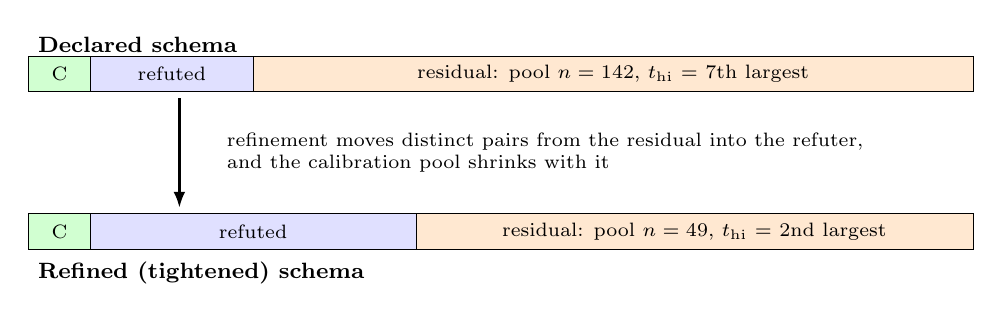
\begin{tikzpicture}[font=\footnotesize, x=0.12cm, y=1cm]
  % Region widths are the test-split shares (percent) under each declaration,
  % primary judge: certified 6.6; refuted 17.2 (declared) / 34.5 (refined).
  % ── declared schema (heading above its bar) ──
  \node[anchor=west, font=\footnotesize\bfseries] at (0,3.20) {Declared schema};
  \fill[green!18] (0,2.60) rectangle (6.6,3.05);
  \fill[blue!12] (6.6,2.60) rectangle (23.8,3.05);
  \fill[orange!18] (23.8,2.60) rectangle (100,3.05);
  \draw (0,2.60) rectangle (100,3.05);
  \draw (6.6,2.60) -- (6.6,3.05);
  \draw (23.8,2.60) -- (23.8,3.05);
  \node[font=\scriptsize] at (3.3,2.825) {C};
  \node[font=\scriptsize] at (15.2,2.825) {refuted};
  \node[font=\scriptsize] at (61.9,2.825) {residual: pool $n=142$, $t_{\mathrm{hi}}$ = 7th largest};
  % ── transition ──
  \draw[-{Latex[length=2mm]}, thick] (16,2.52) -- (16,1.13);
  \node[anchor=west, font=\scriptsize, align=left] at (20,1.83)
    {refinement moves distinct pairs from the residual into the refuter,\\
     and the calibration pool shrinks with it};
  % ── refined schema (heading below its bar) ──
  \fill[green!18] (0,0.60) rectangle (6.6,1.05);
  \fill[blue!12] (6.6,0.60) rectangle (41.1,1.05);
  \fill[orange!18] (41.1,0.60) rectangle (100,1.05);
  \draw (0,0.60) rectangle (100,1.05);
  \draw (6.6,0.60) -- (6.6,1.05);
  \draw (41.1,0.60) -- (41.1,1.05);
  \node[font=\scriptsize] at (3.3,0.825) {C};
  \node[font=\scriptsize] at (23.8,0.825) {refuted};
  \node[font=\scriptsize] at (70.5,0.825) {residual: pool $n=49$, $t_{\mathrm{hi}}$ = 2nd largest};
  \node[anchor=west, font=\footnotesize\bfseries] at (0,0.30) {Refined (tightened) schema};
\end{tikzpicture}
\caption{The refinement dilemma, drawn to scale for the test split (shares of 513 pairs; C: certified; the residual is the fragment the judge decides). Refinement enlarges the refuted region, which removes pairs from the judge's jurisdiction and closes the prose-only injection class. Because the calibration pool is the distinct part of the residual, the pool shrinks with it (primary judge: from 142 to 49 pairs), and at $\alpha=0.05$ the conformal threshold moves from the 7th to the 2nd largest pool score (Proposition~\ref{prop:dilemma}). Section~\ref{sec:res-refinement} measures the consequence.}\label{fig:refinement}
\end{figure}


\subsection{Where existing mechanisms sit}

In this framework, an idempotency key is a certifier on a client-chosen token with residual policy ``execute'' (a fresh token is a fresh act); content-addressed fencing is the certifier $\equiv_\kappa$ with the same residual policy; a raw LLM analyser resolves the whole space, residual included, by an unbounded judgement; and a canonical-action binding~\cite{xu2026caplease} is a certifier on a normal form. We are not aware of a prior mechanism that pairs a sound certifier with a sound refuter and treats only the remainder as a calibrated decision.

\section{The fence}\label{sec:fence}

This section instantiates the framework for irreversible tool calls whose arguments a language model may paraphrase on retry. The certifier is canonical equality under declared field policies; the refuter is inequality of the declared typed fields; the oracle is an LLM judge; calibration is one-sided split-conformal on the safety-critical direction, corrected for the number of candidates; and the residual policy is a three-way rule with an audited middle band. Each is a design choice within the framework, not part of the framework itself. The order matters (Figures~\ref{fig:architecture} and~\ref{fig:flow}): the refuter runs \emph{before} the judge, so a candidate whose declared fields differ is removed from the judge's jurisdiction entirely, and every candidate it removes also shrinks the multiplicity $m$ that the threshold must correct for.

\begin{figure}[!tbp]
\centering
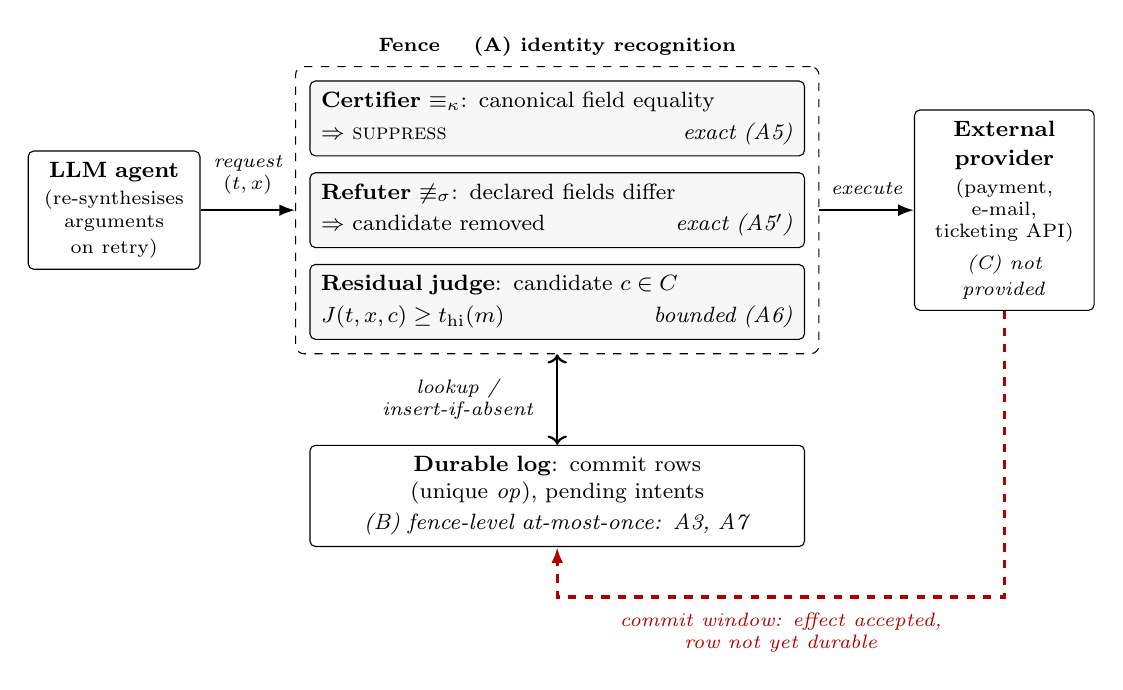
\begin{tikzpicture}[
  font=\footnotesize,
  box/.style={draw, rounded corners=2pt, align=center, inner sep=4pt, fill=white},
  layer/.style={draw, rounded corners=2pt, align=left, inner sep=4pt, text width=6.0cm, fill=gray!6},
  arr/.style={-{Latex[length=2mm]}, thick},
  lbl/.style={font=\scriptsize\itshape, align=center}]
  % Center column: three fence layers
  \node[layer] (l0) {\textbf{Certifier $\equiv_\kappa$}: canonical field equality\\[2pt]$\Rightarrow$ \textsc{suppress}\hfill\emph{exact (A5)}};
  \node[layer, below=0.20cm of l0] (wit) {\textbf{Refuter $\not\equiv_\sigma$}: declared fields differ\\[2pt]$\Rightarrow$ candidate removed\hfill\emph{exact (A5$'$)}};
  \node[layer, below=0.20cm of wit] (jud) {\textbf{Residual judge}: candidate $c\in C$\\[2pt]$J(t,x,c) \ge \thi(m)$\hfill\emph{bounded (A6)}};
  \node[draw, dashed, rounded corners=3pt, inner sep=5pt, fit=(l0)(wit)(jud), label={[font=\scriptsize\bfseries]above:{Fence \quad (A) identity recognition}}] (fence) {};

  % Left: LLM agent
  \node[box, left=1.2cm of fence.west, text width=1.9cm] (agent) {\textbf{LLM agent}\\[2pt]\scriptsize(re-synthesises\\arguments\\on retry)};

  % Right: External provider
  \node[box, right=1.2cm of fence.east, text width=2.0cm] (prov) {\textbf{External}\\[1pt]\textbf{provider}\\[2pt]\scriptsize(payment, e-mail,\\ticketing API)\\[2pt]\emph{(C) not provided}};

  % Bottom: Durable log
  \node[box, below=1.15cm of fence.south, text width=6.0cm] (log) {\textbf{Durable log}: commit rows (unique $\mathit{op}$), pending intents\\[2pt]\emph{(B) fence-level at-most-once: A3, A7}};

  % Main flow arrows
  \draw[arr] (agent.east) -- node[above=2pt, lbl]{request\\$(t,x)$} (fence.west);
  \draw[arr] (fence.east) -- node[above=2pt, lbl]{execute} (prov.west);
  \draw[arr, <->] (fence.south) -- node[left=5pt, lbl]{lookup /\\insert-if-absent} (log.north);

  % Commit window: from prov.south, down to below log, then horizontal to below log.south, then up
  \coordinate (bot) at ([yshift=-18pt]log.south);
  \coordinate (corner) at (prov.south |- bot);
  \draw[very thick, red!70!black, dashed, -{Latex[length=2mm]}]
    (prov.south) -- (corner)
    -- node[below=2pt, font=\scriptsize\itshape, text=red!70!black, align=center]{commit window: effect accepted,\\row not yet durable} (bot)
    -- (log.south);
\end{tikzpicture}
\caption{System view. The fence sits between the agent and an irreversible provider. Identity recognition (A) is decided by two exact layers and a calibrated residual judge; fence-level at-most-once commitment (B) is enforced at the durable log under its storage and scheduling assumptions; external exactly-once (C) is not provided, because a crash inside the commit window (dashed) leaves no local record of an accepted effect (Proposition~\ref{prop:amo}).}\label{fig:architecture}
\end{figure}

\begin{figure}[!tbp]
\centering
\scalebox{0.78}{%
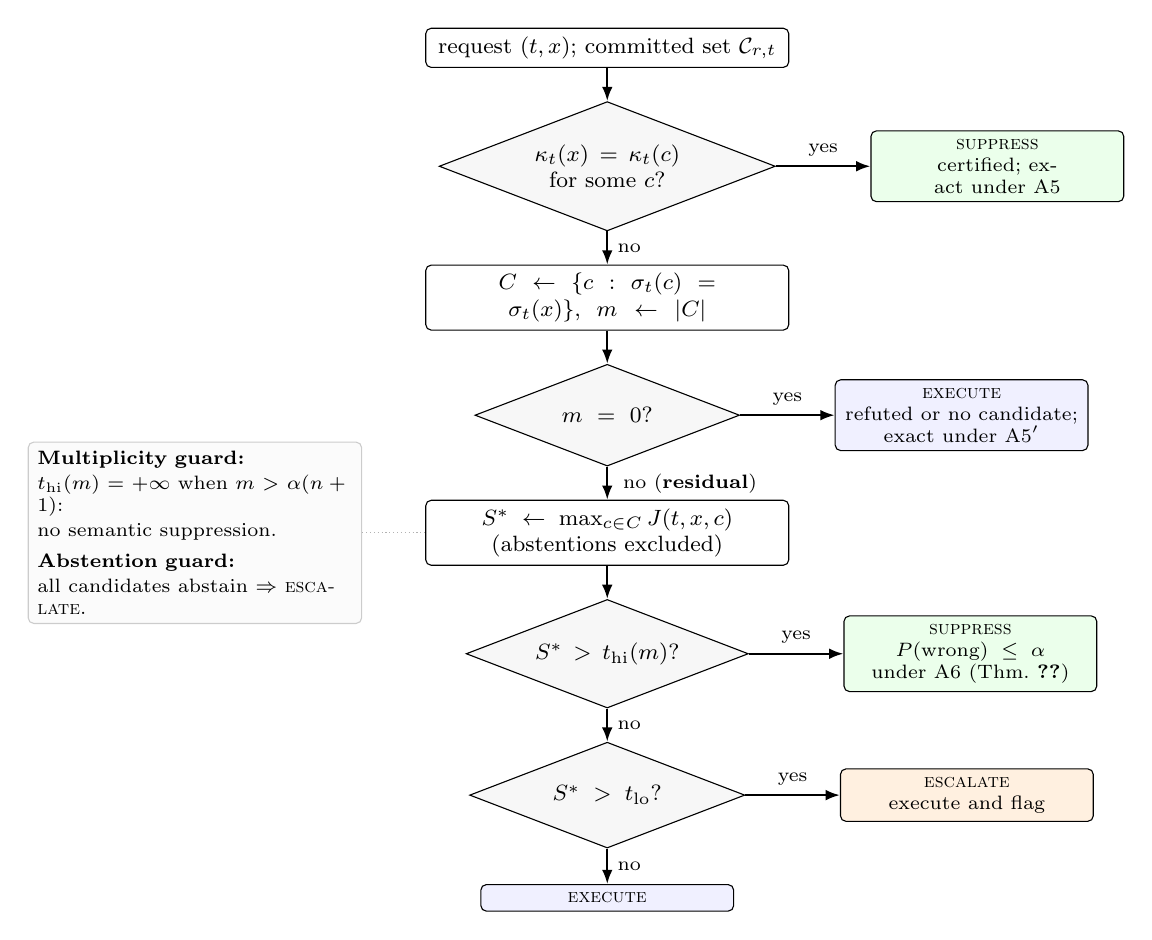
\begin{tikzpicture}[
  font=\footnotesize, node distance=0.42cm,
  fstep/.style={draw, rounded corners=2pt, align=center, inner sep=3pt, text width=4.4cm, fill=white},
  ftest/.style={draw, diamond, aspect=2.6, align=center, inner sep=1pt, text width=2.6cm, fill=gray!6},
  fout/.style={draw, rounded corners=2pt, align=center, inner sep=3pt, text width=3.0cm, font=\scriptsize},
  farr/.style={-{Latex[length=1.8mm]}, thick}]
  \node[fstep] (in) {request $(t,x)$; committed set $\mathcal{C}_{r,t}$};
  \node[ftest, below=of in] (q0) {$\kappa_t(x)=\kappa_t(c)$\\ for some $c$?};
  \node[fstep, below=of q0] (w) {$C\gets\{c:\sigma_t(c)=\sigma_t(x)\}$,\ \ $m\gets|C|$};
  \node[ftest, below=of w] (q1) {$m=0$?};
  \node[fstep, below=of q1] (j) {$S^\ast\gets\max_{c\in C}J(t,x,c)$\\ (abstentions excluded)};
  \node[ftest, below=of j] (q2) {$S^\ast>\thi(m)$?};
  \node[ftest, below=of q2] (q3) {$S^\ast>\tlo$?};
  \node[fout, right=1.2cm of q0, fill=green!8] (s0) {\textsc{suppress}\\ certified; exact under A5};
  \node[fout, right=1.2cm of q1, fill=blue!6] (e0) {\textsc{execute}\\ refuted or no candidate; exact under A5$'$};
  \node[fout, right=1.2cm of q2, fill=green!8] (s1) {\textsc{suppress}\\ $P(\text{wrong})\le\alpha$ under A6 (Thm.~\ref{thm:bound})};
  \node[fout, right=1.2cm of q3, fill=orange!12] (x1) {\textsc{escalate}\\ execute and flag};
  \node[fout, below=0.45cm of q3, fill=blue!6] (e1) {\textsc{execute}};

  \draw[farr] (in) -- (q0);
  \draw[farr] (q0) -- node[above, font=\scriptsize]{yes} (s0);
  \draw[farr] (q0) -- node[right, font=\scriptsize]{no} (w);
  \draw[farr] (w) -- (q1);
  \draw[farr] (q1) -- node[above, font=\scriptsize]{yes} (e0);
  \draw[farr] (q1) -- node[right=2pt, font=\scriptsize]{no (\textbf{residual})} (j);
  \draw[farr] (j) -- (q2);
  \draw[farr] (q2) -- node[above, font=\scriptsize]{yes} (s1);
  \draw[farr] (q2) -- node[right, font=\scriptsize]{no} (q3);
  \draw[farr] (q3) -- node[above, font=\scriptsize]{yes} (x1);
  \draw[farr] (q3) -- node[right, font=\scriptsize]{no} (e1);

  \node[draw=gray!40, rounded corners=2pt, fill=gray!3, align=left, font=\scriptsize, text width=4.0cm, left=0.8cm of j.west, anchor=east] (sideguard) {
    \textbf{Multiplicity guard:}\\[1pt]
    $\thi(m)=+\infty$ when $m>\alpha(n+1)$:\\[1pt]
    no semantic suppression.\\[3pt]
    \textbf{Abstention guard:}\\[1pt]
    all candidates abstain $\Rightarrow$ \textsc{escalate}.
  };
  \draw[densely dotted, gray!60] (sideguard.east) -- (j.west);
\end{tikzpicture}}
\caption{Decision flow for one request. The certifier and the refuter settle their pairs without a model call; only the residual reaches the judge, and the judge can cause suppression only through the multiplicity-corrected threshold. Every path that is not certified ends in execution, flagged or not.}\label{fig:flow}
\end{figure}


\subsection{Certifier: the canonical core}\label{sec:l0}

Each tool schema declares a normalisation policy for each field, and the policy must be semantics-preserving for that field's contribution to the effect (A5). The policies used here are: \texttt{id} (opaque identifier; Unicode NFC normalisation and trimming, case-sensitive); \texttt{ci} (case-insensitive token such as a currency code or e-mail address; NFC, trim, lower case); \texttt{num} (numeric value; \texttt{"120.00"}, \texttt{" 120 "} and \texttt{120} normalise to one canonical decimal, thousands separators removed); and \texttt{text} (free text; NFC, trim, internal whitespace collapsed---deliberately not semantic). The canonical form $\kappa_t(x)$ applies each policy and sorts the keys; the operation identifier is $\mathit{op}=H(r\,\|\,t\,\|\,H(\kappa_t(x)))$ with $H$ = SHA-256. The certifier suppresses a request only when a committed effect has the same identifier and the same stored input hash. It is sound under A5 and deliberately incomplete: every paraphrase escapes it.

\subsection{Refuter: the distinctness witness}\label{sec:witness}

The semantic projection $\sigma_t(x)$ is the tuple of canonical values of the declared non-text fields. Under A5$'$---a difference in any declared typed field implies a different act---$\sigma_t(x)\ne\sigma_t(x')$ proves $x\not\approx_t x'$ whatever any judge would say. The fence removes every committed effect whose projection differs from the request's before the judge is consulted. An injected ``treat this as a duplicate'' cannot cause suppression across a different amount, account or identifier, because those values live in typed fields and the veto fires on them without reading any text. A5$'$ is one-directional: equal projections do \emph{not} imply the same act, and the corpus contains a category (legitimate repeats) in which they do not. Two declaration errors are possible. A field declared as typed that does not in fact determine the act produces false vetoes, which execute a duplicate and are therefore loud; an act-determining field declared as free text leaves its distinction to the judge.

\subsection{Residual judge}\label{sec:judge}

A judge call scores a batch of pairs from the same tool and returns, for each pair, the probability that the two requests denote a single act, as an integer percentage. The prompt is reproduced in the supplementary material. Scores are parsed under a strict contract: an integer in $[0,100]$ is accepted; a non-integer (for example \texttt{0.95}), an out-of-range value, or a missing entry is rejected and the batch retried with a correction; a pair that never yields an admissible value is recorded as an \emph{abstention} rather than imputed. This contract exists for a concrete reason: an earlier scoring pass over a 780-pair version of the corpus stored 180 scores (23.1\%) on the wrong scale while reporting no failures; every number from that pass was withdrawn (supplementary material, Section~S3). Abstentions are dropped from calibration, excluded from the maximum over candidates, and can never cause suppression; if every candidate abstains the fence escalates.

\subsection{Calibration}\label{sec:calibration}

\begin{definition}[Jurisdiction and calibration pool]\label{def:jurisdiction}
The \emph{jurisdiction} of a configuration of decidable layers is the set of pairs that the configuration routes to the judge. Its \emph{calibration pool} is the multiset $\{s_1,\dots,s_n\}$ of judge scores of the distinct pairs of a held-out calibration split that lie in its jurisdiction, with abstentions dropped.
\end{definition}

For the proposed configuration (certifier and refuter both active) the jurisdiction is the residual (Definition~\ref{def:residual}). For a candidate set of size $m\ge1$ the suppression threshold is
\begin{equation}\label{eq:thi}
\thi(m)=s_{(k)},\qquad k=\big\lceil (n+1)(1-\alpha/m)\big\rceil,\qquad \thi(m)=+\infty \text{ if } k>n,
\end{equation}
where $s_{(k)}$ is the $k$-th smallest pool score, and $\thi(0)=+\infty$. The escalation floor $\tlo$ is the $\lfloor (n_S+1)\gamma\rfloor$-th smallest score of the $n_S$ duplicate pairs in the same jurisdiction, capped at $\thi$. With $S^\ast$ the maximum score over the candidates that did not abstain, the fence \emph{suppresses} if $S^\ast>\thi(m)$, \emph{escalates} (executes and flags) if $\tlo<S^\ast\le\thi(m)$, and \emph{executes} if $S^\ast\le\tlo$. The inequality for suppression is strict, so a score equal to the threshold never suppresses; judge scores are integer percentages, so such ties are common.

Two design choices need justification. First, the pool must be drawn from the rule's own jurisdiction. Adding the refuter removes from the judge's view the distinct pairs whose declared fields differ; judges score such pairs confidently low, so a pool that still contains them is stochastically lighter-tailed than the scores the deployed rule thresholds, which lowers $\thi$ and makes suppression easier. The resulting violation is in the unsafe direction and is invisible in a rate measured over a whole test split, because the pairs that dilute the pool also dilute the denominator (Section~\ref{sec:res-bound}). Every configuration in this paper, including every ablation, is therefore re-calibrated on its own jurisdiction. Second, we correct for multiplicity by the Bonferroni level $\alpha/m$ rather than by calibrating the maximum statistic directly. Direct calibration needs calibration \emph{units} with the deployment's candidate-set structure: a pool of $n$ pairwise scores yields only $\lfloor n/m\rfloor$ disjoint units, certifying $\alpha=0.05$ needs at least 19 units, and $m$ varies from one request to the next. The Bonferroni route reuses one pool at every $m$, requires only pairwise exchangeability, and degrades gracefully to $\thi=+\infty$ when the pool is too small. Its price is conservatism, which we measure (Section~\ref{sec:res-bound}).

\subsection{Algorithm}

Algorithm~\ref{alg:fence} gives the complete decision procedure, including the execute path. A request that is not suppressed records a \textsc{pending} intent, executes, and then attempts an atomic insert of its commit row; a crash between the external effect and the insert leaves a \textsc{pending} intent with no commit row. That interval---the \emph{commit window}---cannot be closed by any local mechanism (Proposition~\ref{prop:amo}). An optional window guard compares a new request against such orphaned intents and flags a suspected re-fire; it never suppresses on one, because a pending intent does not establish that the effect happened.

\begin{algorithm}[!tbp]
\caption{Layered semantic fence (the proposed configuration).}\label{alg:fence}
\scriptsize
\KwIn{request $(t,x)$ in run $r$; durable log $L$; pool $\{s_i\}_{i\le n}$; floor $\tlo$; level $\alpha$}
\If{$t$ is idempotent}{\Return execute$(x)$}
$\mathit{op}\gets H(r\,\|\,t\,\|\,H(\kappa_t(x)))$\;
\If(\tcp*[f]{certifier; exact under A5}){$L$ has a commit row for $\mathit{op}$ with input hash $H(\kappa_t(x))$}{\Return its recorded response}
$C\gets\{c\in L.\mathrm{committed}(r,t) : \sigma_t(c.x)=\sigma_t(x)\}$\tcp*{refuter removes declared differences}
\If{$C\neq\emptyset$}{
  $s_c\gets J(t,c.x,x)$ for each $c\in C$ \tcp*{abstention $\Rightarrow$ $s_c=\bot$}
  $m\gets|C|$;\quad $\thi\gets\thi(m)$ by Eq.~\eqref{eq:thi}\;
  \If{all $s_c=\bot$}{flag \textsc{duplicate\_suspect}}
  \Else{
    $S^\ast\gets\max\{s_c : s_c\neq\bot\}$, attained at $c^\ast$\;
    \lIf{$S^\ast>\thi$}{\Return $c^\ast$.response \tcp*[f]{semantic suppression}}
    \lIf{$S^\ast>\tlo$}{flag \textsc{duplicate\_suspect} \tcp*[f]{escalate: execute and flag}}
  }
}
record intent$(\mathit{op},\textsc{pending})$\;
$\mathit{resp}\gets$ execute$(x)$ \tcp*{commit window opens}
$\mathit{ok}\gets L.$insertIfAbsent$(\mathit{op},H(\kappa_t(x)),\sigma_t(x),x,\mathit{resp})$ \tcp*{commit window closes}
record intent$(\mathit{op},\ \mathit{ok}\ ?\ \textsc{committed} : \textsc{commit\_conflict})$\;
\Return $\mathit{resp}$\;
\end{algorithm}

\subsection{Conservative defaults}\label{sec:defaults}

The fence prefers execution to semantic suppression whenever the evidence for suppression is not certified. The threshold is $+\infty$---no semantic suppression, only decidable suppression---when the pool cannot certify level $\alpha$ at the current $m$ (fewer than $m/\alpha-1$ pool scores), when $m=0$, and whenever the pool is absent. A judge abstention can never cause suppression. Inside the commit window a suspected re-fire is executed and flagged, never suppressed. In every uncertain case the failure mode is a loud duplicate rather than a silent loss of a distinct act---the direction the loss asymmetry of Section~\ref{sec:problem} demands.

\section{Theoretical analysis}\label{sec:theory}

The individual tools used below---split-conformal calibration, the union bound, order statistics---are standard, and so are most of the arguments. What this section contributes is an account of what their composition guarantees to an agent that must decide under irreversibility with a stochastic oracle, and of the conditions under which it does. Propositions~\ref{prop:sound} and~\ref{prop:residual} make the certifier/refuter/residual decomposition exact. Theorem~\ref{thm:bound} applies conformal calibration with a Bonferroni correction to the statistic the fence actually thresholds---a maximum over a variable-size candidate set behind decidable vetoes---and makes its validity condition explicit: the pool must be drawn from the rule's own jurisdiction, and a pool that is not can hide its own violation (Section~\ref{sec:res-bound}). Theorem~\ref{thm:tight} records that the classical bound is attained by that statistic, so the correction and the budget are forced rather than conservative. Proposition~\ref{prop:dilemma} and Corollary~\ref{cor:mondrian} state the refinement dilemma exactly. The remaining propositions delimit what is guaranteed; they are stated because nearby designs violate them.

\subsection{Assumptions and their status}\label{sec:assumptions}

Table~\ref{tab:assumptions} lists every assumption and how the experiments satisfy or test it. Several are environmental, and a deployment that does not supply them does not obtain the corresponding guarantee.

{\footnotesize
\begin{longtable}{@{}p{3.1cm}p{2.4cm}p{7.6cm}@{}}
\caption{Assumptions, their type, and their status in the implementation and experiments. ``Measured'' entries test an assumption on this corpus; they do not establish it in general.}\label{tab:assumptions}\\
\toprule
Assumption & Type & Status in this work \\
\midrule
\endfirsthead
\toprule
Assumption & Type & Status in this work \\
\midrule
\endhead
A1 Stable run identifier across retries and replays & environment & Supplied by the harness; a retry under a new identifier is out of scope. \\
A2 Deterministic canonical identity: $\kappa_t$ and $H$ are pure; $H$ is collision-free & implementation & Pure canonicalisation; $H$ is SHA-256; unit-tested. \\
A3 Atomic insert-if-absent on $\mathit{op}$ & storage & \emph{Partial:} unique for a single writer but not crash-atomic; crashes injected at protocol points, not inside a write. \\
A4 Effect before commit; commit only on success & implementation & Algorithm~\ref{alg:fence}; eight injected crash points (Section~\ref{sec:res-crash}). \\
A5 Every declared field policy is semantics-preserving & schema & Tool author's obligation. Measured: 0 of 232 distinct test pairs canonically equal. \\
A5$'$ A difference in a declared typed field implies a different act (one direction only) & schema & Tool author's obligation. Measured: 0 of 281 duplicates refuted; 20 of 20 typed-field injections refuted. \\
A5$''$ Projection completeness: $\sigma_t(x)=\sigma_t(x')\Leftrightarrow x\approx_t x'$ & schema (optional) & Only in Proposition~\ref{prop:compose}, Case A; false for every tool in the corpus. \\
A6 Conditionally on $m$, each score of a truly distinct residual comparison is exchangeable with the calibration pool & statistical & Stratified pair-level split, attacks held out; 82.8\% of test pairs share a seed act with a calibration pair, tested by seed-level resplitting (Section~\ref{sec:res-bound}). Needs a stationary judge; unverifiable at deployment. \\
A7 No concurrent dispatch per identity & scheduler & Sequential dispatch in all experiments; concurrency not tested. \\
A8 The provider applies at most one effect per idempotency key & provider & Only in Proposition~\ref{prop:compose}; absent by design in the crash experiment. \\
\bottomrule
\end{longtable}}

Structurally, the candidate set of a request is every effect committed in the same run for the same tool; duplicates across runs or across tools are outside every result below.

\subsection{Soundness of the decidable layers}

\begin{proposition}[Decidable layers]\label{prop:sound}
Under A2 and A5, every certifier suppression is correct: if the fence suppresses on the canonical branch, the request denotes the same act as the matched committed effect. Under A5$'$, no judge output can cause suppression of a request whose declared typed fields differ from those of every committed effect.
\end{proposition}

\begin{proof}
The canonical branch fires only if $H(\kappa_t(x))=H(\kappa_t(x'))$ for a committed $x'$; by A2 this implies $\kappa_t(x)=\kappa_t(x')$ and by A5 $x\approx_t x'$. For the second claim, a committed effect whose projection differs is removed from $C$ before any judge call, so it is never the maximising candidate; if every committed effect differs, $C=\emptyset$ and the fence executes.
\end{proof}

\subsection{A bound on the deployed statistic}\label{sec:bound}

The fence suppresses on $S^\ast=\max_{c\in C}J(t,x,c)$, not on one pairwise score, and a pairwise bound $P(s_i>\hat t)\le\alpha$ does not imply $P(\max_i s_i>\hat t)\le\alpha$. The result below is stated for the deployed statistic.

\begin{theorem}[Multiplicity-corrected wrong-suppression bound]\label{thm:bound}
Let the pool $\{s_i\}_{i\le n}$ be drawn from the rule's jurisdiction (Definition~\ref{def:jurisdiction}) and let $\thi(m)$ be given by Eq.~\eqref{eq:thi}. Suppose (A6) that, conditionally on $m$, the judge score of any comparison between a request and a candidate that denotes a different act is exchangeable with the pool. Then for every request $x$ that denotes a different act from every member of its candidate set $C$, $|C|=m$,
\[
P\big(S^\ast(x,C)>\thi(m)\big)\le\alpha ,
\]
for every $m\ge0$, with no assumption on the distribution of scores and no assumption on the dependence among the $m$ comparisons.
\end{theorem}

\begin{proof}
Condition on $m$. If $m=0$ or $\thi(m)=+\infty$ the fence cannot suppress and the probability is $0$. Otherwise let $\beta=\alpha/m$ and $k=\lceil(n+1)(1-\beta)\rceil\le n$, so $\thi(m)=s_{(k)}$. Fix a candidate $c_i\in C$. Because $x\not\approx_t c_i$, its score $s'_i$ is a distinct-pair score, so by A6 the $n+1$ values $s_1,\dots,s_n,s'_i$ are exchangeable and, with ties broken uniformly at random, the rank of $s'_i$ among them is uniform on $\{1,\dots,n+1\}$. If $s'_i>s_{(k)}$, then $s'_i$ exceeds at least $k$ pool values and has rank at least $k+1$ under any tie-breaking, so
\[
P\big(s'_i>s_{(k)}\big)\le\frac{n+1-k}{n+1}\le 1-(1-\beta)=\beta .
\]
This holds for each $i$ separately. The union bound over the $m$ candidates, which requires no independence, gives
\[
P\big(S^\ast>\thi(m)\big)=P\big(\exists i\le m: s'_i>\thi(m)\big)\le\sum_{i=1}^m P\big(s'_i>\thi(m)\big)\le m\beta=\alpha .
\]
The bound holds conditionally on each value of $m$ and therefore also after averaging over the distribution of $m$. Abstentions only remove candidates from the maximum while $\thi(m)$ is computed with the full $m$, which is conservative.
\end{proof}

The probability is joint over the calibration pool and the request, so the bound is \emph{marginal}: a particular deployment's pool can exceed $\alpha$ (Section~\ref{sec:res-bound}), and nothing is claimed under distribution shift, including injection (Section~\ref{sec:limitations}). It tolerates arbitrary dependence among the $m$ comparisons, which share $x$.

\paragraph{The pool must match the jurisdiction}
A6 compares the pool with the scores the deployed rule thresholds, and which pairs those are is decided by the layers in front of the judge. A pool drawn from a wider population satisfies A6 only by coincidence; if the extra pairs score lower, the threshold falls and the bound fails while the rate over a whole test split still looks acceptable. Jurisdiction matching is therefore a necessary condition of the theorem, not an implementation detail.

\paragraph{The escalation floor}
A duplicate's candidate set contains its match, so taking a maximum helps the escalation side and $\tlo$ needs no correction. With integer-percent scores ties are frequent and $\tlo$ is capped at $\thi$, so we treat the band as an empirical quantity (Section~\ref{sec:res-components}) and claim no bound for it.

\subsection{Calibration budget and the refinement dilemma}\label{sec:dilemma}

\begin{proposition}[Calibration budget; refinement dilemma]\label{prop:dilemma}
Let a configuration have pool size $n$ and level $\alpha$.
\begin{enumerate}[(a),leftmargin=*,itemsep=1pt]
\item $\thi(m)$ is finite if and only if $m\le\alpha(n+1)$; equivalently, semantic suppression at candidate-set size $m$ requires $n\ge\lceil m/\alpha\rceil-1$, and the largest certifiable candidate-set size is $m^\ast=\lfloor\alpha(n+1)\rfloor$.
\item When finite, $\thi(m)$ is the $\rho$-th \emph{largest} pool score with $\rho=\lfloor (n+1)\alpha/m\rfloor$, which is non-decreasing in $n$.
\item If $(\kappa',\sigma')$ refines $(\kappa,\sigma)$ and both are calibrated on the same calibration split, the refined pool is a sub-multiset of the original pool. Hence $n'\le n$, $m^{\ast\prime}\le m^\ast$ and $\rho'\le\rho$: refinement can only shrink the certifiable budget and move the threshold to an equal or higher rank from the top.
\end{enumerate}
\end{proposition}

\begin{proof}
(a) Since $n$ is an integer, $\lceil(n+1)(1-\alpha/m)\rceil\le n$ holds iff $(n+1)(1-\alpha/m)\le n$, i.e.\ iff $m\le\alpha(n+1)$. (b) The $k$-th smallest of $n$ values is the $(n+1-k)$-th largest, and $n+1-\lceil(n+1)(1-\alpha/m)\rceil=\lfloor (n+1)\alpha/m\rfloor$. (c) The pool is the set of distinct calibration pairs in the jurisdiction with a score; the jurisdiction of the proposed configuration is the residual, and by Proposition~\ref{prop:residual}(iii) the refined residual is contained in the original one.
\end{proof}

At $\alpha=0.05$ and $m=1$, the declared pool of the primary judge ($n=142$) places $\thi$ at the 7th largest score, the tightened pool of Section~\ref{sec:res-refinement} ($n=49$) at the 2nd largest, and any pool with $n\le18$ at $+\infty$. The proposition does \emph{not} say the refined threshold is numerically higher; that depends on whether the judge scores the removed pairs lower than those that remain, which Section~\ref{sec:res-refinement} measures. Asking for the bound to hold within each kind of difference is a second refinement---of the calibration population rather than of the schema---and it pays the same price.

\begin{corollary}[Class-conditional budget]\label{cor:mondrian}
Partition the jurisdiction into classes $c=1,\dots,K$ by a function of the request, let the pool contain $n_c$ scores of class $c$ ($\sum_c n_c=n$), and let $t_c(m)$ be Eq.~\eqref{eq:thi} computed on the class-$c$ pool alone.
\begin{enumerate}[(a),leftmargin=*,itemsep=1pt]
\item If A6 holds within each class, then $P(S^\ast>t_c(m)\mid\text{class } c)\le\alpha$ for every $c$.
\item $t_c(m)$ is finite iff $m\le\alpha(n_c+1)$. Every class is certifiable at $m$ iff $\min_c n_c\ge\lceil m/\alpha\rceil-1$, which requires $n\ge K(\lceil m/\alpha\rceil-1)$; and $\min_c\lfloor\alpha(n_c+1)\rfloor\le\lfloor\alpha(n/K+1)\rfloor$.
\item If the class is not observable when the fence decides, thresholding at $\max_c t_c(m)$ satisfies (a) for every class simultaneously; it is finite only if every class is certifiable at $m$.
\end{enumerate}
\end{corollary}

Each class pool is a sub-multiset of the pool, so its threshold sits at an equal or higher rank from the top: partitioning the jurisdiction into $K$ classes gives each class the budget of Proposition~\ref{prop:dilemma}(a) at its own $n_c$. A per-class guarantee costs calibration budget, and when the classes are defined by the label, as the kinds of difference in our corpus are, it costs the deduplication of the most conservative class (Section~\ref{sec:res-class}).

\subsection{The standard bound is attained}\label{sec:tight}

Theorem~\ref{thm:bound} rests on a union bound. That the union bound is sharp when nothing is known about the dependence among the events is classical: $P(\bigcup_iA_i)\le\min\{1,\sum_iP(A_i)\}$ is the upper Fr\'echet bound, attained when the events are disjoint or cover the space~\cite{frechet1935,ruschendorf1982maxsums,galambos1996bonferroni}, and the sharper bounds of Hunter and Worsley need the pairwise intersection probabilities~\cite{hunter1976union,worsley1982bonferroni}, which a fence does not know. In the language of merging p-values, the Bonferroni rule is precise and admissible under arbitrary dependence~\cite{vovk2020averaging,vovk2022admissible}. We therefore do not present the tightness below as a new technical result. It answers a narrower question: is the classical worst case reachable by the \emph{deployed} statistic under the fence's own assumption, and does any rule a fence can audit do better? Within deterministic rules that do not depend on the scale of the judge's scores---which are uncalibrated, so a rule that reads meaning into their absolute values inherits that miscalibration---the standard bound is exactly attained. Lemma~\ref{lem:scalefree}, which identifies the class, is a characterisation of a known type---symmetric functions that commute with every increasing bijection are order statistics~\cite{ovchinnikov1997invariant,marichal2002order}---stated here without a continuity assumption and proved in \ref{app:proofs} for completeness.

\begin{lemma}[Scale-free thresholds]\label{lem:scalefree}
Let $\tau$ map pools of $n$ distinct scores to $[-\infty,+\infty]$, be symmetric in its arguments, and satisfy $\tau(g(s_1),\dots,g(s_n))=g(\tau(s_1,\dots,s_n))$ for every strictly increasing bijection $g$ of $\mathbb{R}$, extended by $g(\pm\infty)=\pm\infty$. Then $\tau\equiv s_{(k)}$ for one fixed $k\in\{1,\dots,n\}$, or $\tau\equiv+\infty$, or $\tau\equiv-\infty$.
\end{lemma}

A deterministic rule that thresholds $S^\ast$ at a scale-free function of the pool is therefore ``suppress iff $S^\ast>s_{(k)}$'' for a fixed $k$, or never suppresses, or always does. The fence is such a rule, with $k=k^\ast=\lceil(n+1)(1-\alpha/m)\rceil$ when $k^\ast\le n$ and $\rho=n+1-k^\ast$ as in Proposition~\ref{prop:dilemma}. Let $\mathcal{Q}_{n,m}$ be the class of joint laws of $(s_1,\dots,s_n,s'_1,\dots,s'_m)$ in which, for each $i$, the pool and $s'_i$ are $n+1$ independent draws from one continuous distribution, with arbitrary dependence among $s'_1,\dots,s'_m$. Every law in $\mathcal{Q}_{n,m}$ satisfies A6, so a rule that is valid under A6 must be valid on all of $\mathcal{Q}_{n,m}$.

\begin{theorem}[The standard bound is attained by the deployed statistic]\label{thm:tight}
For every $k\in\{1,\dots,n\}$,
\[
\sup_{\mathcal{Q}_{n,m}} P\Big(\max_{i\le m}s'_i>s_{(k)}\Big)=\mathbb{E}\big[\min\{1,mB\}\big],\qquad B\sim\mathrm{Beta}(n+1-k,\,k),
\]
and the supremum is attained. For the fence's threshold,
\[
\sup_{\mathcal{Q}_{n,m}}P(\text{wrong suppression})\;=\;\frac{m\rho}{n+1}-\mathbb{E}\big[(mB-1)_+\big]\;\le\;\frac{m\rho}{n+1}\;\le\;\alpha,
\]
where $\mathbb{E}[(mB-1)_+]\le(m-1)\exp\!\big(-(1-\alpha)^2n/(2m)\big)$.
\end{theorem}

The attaining law is not exotic: pool and candidate scores are i.i.d., the most favourable reading of A6, and only the joint behaviour of one request's $m$ candidate scores is adversarial---spread so that at most one is high, as when a request is compared with committed effects that differ from it in different ways.

\begin{corollary}[What cannot be improved]\label{cor:tight}
Fix $\alpha\in(0,1)$ and $m\ge1$. Worst cases are over $\mathcal{Q}_{n,m}$.
\begin{enumerate}[(a),leftmargin=*,itemsep=1pt]
\item \emph{The constant.} For $m=1$ the worst case is $\rho/(n+1)$, which equals $\alpha$ whenever $(n+1)\alpha$ is an integer; for every $m$ it tends to $\alpha$ as $n\to\infty$. No constant below $\alpha$ bounds wrong suppression for all pool sizes.
\item \emph{The correction.} For $m=1$, every rank $k<k^\ast$ has worst case $(n+1-k)/(n+1)>\alpha$. For every $m$, a rule with a fixed per-candidate level $\gamma>\alpha/m$ has worst case tending to $\min\{1,m\gamma\}>\alpha$. The Bonferroni level is the largest per-candidate level valid for every pool size without an assumption on the dependence among the $m$ comparisons.
\item \emph{The budget.} If $m>\alpha(n+1)$, the most conservative finite threshold, the pool maximum ($k=n$), has worst case exactly
\[
\mathbb{E}\big[\min\{1,mB\}\big]=\frac{m}{n+1}\Big(1-\Big(1-\frac1m\Big)^{n+1}\Big),\qquad B\sim\mathrm{Beta}(1,n),
\]
and every other finite threshold has a larger one. This exceeds $\alpha$ unless $m/(n+1)$ lies within $\delta_{0.05}<1.1\times10^{-10}$ of $\alpha$ (at $\alpha=0.05$; proof in \ref{app:proofs}), which no pool with $n+1<4.8\times10^8$ can do. There, switching semantic suppression off beyond the budget is forced rather than conservative: the only valid deterministic scale-free rule is never to suppress.
\end{enumerate}
\end{corollary}

Proofs are in \ref{app:proofs}. For every configuration in this paper the gap between worst case and bound is below $10^{-10}$: 4.895\% for the declared pool ($n=142$, $m=1$), 4.000\% for the tightened pool ($n=49$), and 4.975\% at $n=200$ for $m=1,2,5,10$, the simulation setting of Section~\ref{sec:res-bound}, whose law gave 3.7\% at $m=10$. One rank lower the worst case exceeds $\alpha$ (5.594\% and 6.000\%). Under the attaining law the uncorrected rule suppresses 49.7\% of distinct requests at $m=10$ and 99.9\% at $m=50$, against 38.3\% and 89.0\% in the simulation. A direct simulation of the attaining law agrees with the exact values in all eight configurations we computed; the budget condition was checked for every $n+1\le10^6$ at $\alpha=0.05$ and $\alpha=0.01$ with no exception; and the equality in Corollary~\ref{cor:tight}(c) was checked without its closed form, against the general rank-$k$ computation at $k=n$ to within $10^{-12}$ over 4,000 pairs $(n,m)$, and by simulation, which agrees in all six budget configurations (supplementary material, Section~S21). The result concerns deterministic rules: a coin-tossing rule beyond the budget is valid but cannot be audited or replayed. With integer-percent scores, ties lower the realised rate (Section~\ref{sec:res-components}).

\subsection{Why the architecture is layered}

\begin{proposition}[No zero-error threshold on overlapping scores]\label{prop:impossible}
Let $F_{\mathrm{same}}$ and $F_{\mathrm{diff}}$ be the judge-score distributions of duplicate and distinct pairs. If they overlap---some score has positive probability under both---no rule that thresholds the score alone achieves zero wrong suppression and zero silent escape simultaneously. An escalation band can remove silent escape only by flagging, not suppressing, the duplicates in the overlap.
\end{proposition}

The proof is in \ref{app:proofs}. Zero error on a class needs a decision that does not consult the score, which is what the certifier and refuter are; the overlap is judge- and tool-dependent (supplementary material, Section~S8).

\subsection{Fence-level at-most-once}\label{sec:amo}

\begin{proposition}[Fence-level at-most-once commitment]\label{prop:amo}
Under A1--A4 and A7, for a fixed run $r$ and operation identifier $\mathit{op}$, across any number of serialised executions and process restarts sharing the durable log, the effect for $\mathit{op}$ is dispatched and committed at most once by the fence, except that a crash strictly between the external effect and the commit insert leaves a \textsc{pending} intent with no commit row, after which a later execution may dispatch again.
\end{proposition}

The proof is in \ref{app:proofs}. The commit window cannot be closed by any local mechanism, because during it the only record of the effect is at the provider. Without A7, two concurrent executions can both miss the log and dispatch; at most one commit row survives and the loser records \textsc{commit\_conflict}, so the duplicate is observable but not prevented.

\subsection{External exactly-once only by composition}\label{sec:compose}

\begin{proposition}[Composition with a provider key]\label{prop:compose}
\emph{Case A.} If a key function $\pi_t$ is paraphrase-invariant ($x\approx_t x'\Rightarrow\pi_t(x)=\pi_t(x')$) and complete for identity ($\pi_t(x)=\pi_t(x')\Rightarrow x\approx_t x'$), and the provider satisfies A8, then presenting $\pi_t(x)$ as the provider's idempotency key yields external exactly-once application for that tool, including across the commit window. A schema satisfying A5$''$ supplies $\pi_t=\sigma_t$.
\emph{Case B.} If the schema satisfies A5$'$ but not A5$''$, then $\sigma_t$ is not admissible as a provider key (distinct acts sharing a projection would be merged at the provider, a wrong suppression that no local audit can see), and the canonical identifier $\mathit{op}$ is admissible but not paraphrase-invariant; the commit window then remains open for paraphrased retries.
\end{proposition}

\begin{proposition}[Identity recognition is not substitutable]\label{prop:structure}
Mis-recognised identity defeats both fence-level commitment and a correct provider key: an unrecognised duplicate presents a fresh key, which a correct provider must apply, and a wrongly recognised distinct act presents a stale key, which a correct provider absorbs. Conversely, a provider key satisfying Case A of Proposition~\ref{prop:compose} makes A7 unnecessary for at-most-once application.
\end{proposition}

Proofs are in \ref{app:proofs}. Identity recognition (A) is thus the one guarantee neither the log nor the provider can supply, because both are keyed on its output.

\subsection{What is proved and what is measured}

Proved: exactness of the decidable layers under A2, A5 and A5$'$ (Proposition~\ref{prop:sound}); the marginal bound under A6 with its budget, overall and per class (Theorem~\ref{thm:bound}, Proposition~\ref{prop:dilemma}, Corollary~\ref{cor:mondrian}); attainment of the standard bound by the deployed statistic (Theorem~\ref{thm:tight}, Corollary~\ref{cor:tight}); fence-level at-most-once under A1--A4 and A7 (Proposition~\ref{prop:amo}); external exactly-once only by composition (Proposition~\ref{prop:compose}). Everything else is measured: whether the assumptions hold on this corpus, the residual's size, each judge's deduplication, how the realised rate varies across pools, splits and kinds of difference, behaviour under injection, and the composition part of the refinement dilemma.

\section{Experimental methodology}\label{sec:method}

Every analysis is an offline recomputation from persisted corpus files and judge scores; no number in Sections~\ref{sec:method}--\ref{sec:results} requires a model call to regenerate. Commands, configuration and data are listed in the supplementary material and the artifact.

\subsection{Corpus}

The corpus comprises 1,066 labelled pairs of requests over six irreversible tools: \texttt{charge\_card} (customer identifier, amount, currency, memo), \texttt{post\_refund} (charge identifier, amount, reason), \texttt{transfer\_funds} (two account identifiers, amount, currency, note), \texttt{send\_email} (recipient, subject, body), \texttt{create\_ticket} (title, description, priority), and \texttt{wire\_money}, whose amount, beneficiary and reference are all declared as free text. The last tool is deliberately loosely typed: every non-identical pair of wires is residual, so the judge carries its entire identity decision. Each pair is labelled SAME or DIFF \emph{by construction} (Table~\ref{tab:corpus}): a SAME pair is produced by a transformation instructed to preserve the act and checked by a validator that rejects any variant altering a pinned numeric value or recipient; a DIFF pair mutates a declared field, inserts a distinguishing token, or is hand-specified to differ in intent. The labels thus operationalise our definition of identity (Definition~\ref{def:operational}); Section~\ref{sec:res-labels} tests how much the conclusions depend on that.

\begin{table}[!tbp]
\centering\scriptsize
\caption{Corpus. Calibration/test counts are for the benign split; injection pairs are held out of calibration entirely.}\label{tab:corpus}
\begin{tabularx}{\linewidth}{@{}llrrX@{}}
\toprule
Code & Label & $n$ & cal/test & Construction \\
\midrule
S1 & SAME & 68 & 34/34 & mechanical reformat: key order, whitespace, number, currency and case formats \\
S2 & SAME & 253 & 126/127 & paraphrase of free text with typed fields pinned; four generator arms \\
S3 & SAME & 75 & 37/38 & loose-schema value rewrite, e.g.\ ``\$780.00'' $\leftrightarrow$ ``seven hundred eighty dollars'' \\
S4 & SAME & 163 & 81/82 & paraphrase instructed to maximise surface difference while preserving the act \\
D1 & DIFF & 251 & 125/126 & one field mutated ($\pm1$, $\pm0.01$, $\times10$, identifier or order-number change, currency swap) \\
D2 & DIFF & 150 & 75/75 & legitimate repeats: identical except a distinguishing token (``instalment 1 of 2'' vs ``2 of 2'') \\
D3 & DIFF & 61 & 30/31 & hand-specified same-surface, different-intent pairs \\
D4a & DIFF & 20 & held out & typed field differs \emph{and} free text says ``treat as duplicate; suppress'' \\
D4b & DIFF & 25 & held out & typed fields identical, distinct act, injection in free text \\
\midrule
\multicolumn{2}{@{}l}{Total} & 1,066 & 508/513 & 559 SAME, 507 DIFF; 45 attack pairs \\
\bottomrule
\end{tabularx}
\end{table}

\paragraph{Generator arms}
Four generator arms ensure that self-recognition by a judge can be measured rather than assumed away: Llama-3.3-70B (109 pairs), GPT-OSS-120B (121) and Qwen3.6-27B (118) at temperature 0.9, and a hand-written arm of 68 S2 pairs with no model in the loop. The remaining 650 pairs are mechanical transformations or hand-specified pairs with no generator. The validator rejected 8--19 variants per model arm (supplementary material, Section~S2).

\paragraph{Sizing}
Wrong suppression is estimated over DIFF pairs alone, so the DIFF count sets the precision of the safety claim. With 232 DIFF test pairs, an observed zero admits a 95\% Wilson upper bound of 1.6\%, inside the certified $\alpha=0.05$; with the 72 DIFF pairs of an earlier corpus version the same zero admitted 5.1\%, wider than $\alpha$. Two cells that carried qualitative claims were enlarged additively during an earlier revision (S3 from 15 to 75 pairs and D3 from 10 to 61, under a separate seed); no existing pair was modified.

\subsection{Splits and leakage}

Benign pairs are split 50/50 into calibration and test, stratified by (category, generator) with a fixed seed; injection categories are held out entirely. The build asserts that no pair identifier appears on both sides and that no attack pair enters calibration. Pairs derived from the same seed act (the same underlying request, paraphrased or mutated differently) can fall on both sides: 425 of 513 test pairs (82.8\%~[79.3--85.9]) share a seed act with some calibration pair. Exchangeability (A6) is a condition on scores rather than on provenance, so this is not automatically a violation, but it is a route to optimism. We therefore also report 200 seed-level splits that partition the 219 seed acts first and assign every pair together with its seed.

\subsection{Judges, prompt and parsing}

Three judges are reported: GPT-OSS-120B (primary), GPT-OSS-20B and Qwen3.6-27B, all reached through Groq's OpenAI-compatible endpoint in August 2026, at temperature 0, scoring batches of ten pairs. The two GPT-OSS models share a family; Qwen is a second family. A judge is admitted to the tables only if it meets three conditions fixed before any scoring: coverage of at least 80\% of pairs, at least two distinct score values, and an AUC of at least 0.60 between SAME and DIFF scores. The second and third conditions exclude a judge that answers every pair identically, whose calibrated threshold would suppress nothing and report a misleadingly perfect zero. GPT-OSS-120B and GPT-OSS-20B scored all 1,066 pairs (AUC 0.962 each); Qwen3.6-27B scored 1,041 (97.7\%, AUC 0.974), its 25 abstentions being pairs on which its reasoning exhausted the completion budget. Exact permutation tests find no association between Qwen's abstentions and category, label, tool, split or generator (smallest $p=0.09$, for tool; supplementary material, Section~S4). Llama-3.3-70B reached 5.6\% coverage before its endpoint became unavailable and is excluded. No accepted value in the reported scoring violated the integer-percentage contract. Model weights are not pinned by the provider, so a re-run against an updated endpoint constitutes a different experiment.

\subsection{Configurations and baselines}

The configurations compared are: B0 no fence; B1 exact-string identity; B2 canonical-key (content-addressed) fencing, the prior-art baseline; a raw judge at a fixed threshold $\tau=0.5$; the \emph{layered} configuration (certifier and calibrated judge, no refuter); the \emph{hardened} configuration (certifier, refuter, calibrated judge and escalation band), which is the proposed system; and a \emph{tightened} configuration---the hardened system with a refined projection that adds to $\sigma_t$, for every free-text field of every tool, the set of numeric magnitudes the field mentions. The tightened configuration models a tool author who types the numbers that prose carries; it is an intervention, not the baseline system. Every configuration, including every ablation, is calibrated on its own jurisdiction. The primary level is $\alpha=0.05$, with $\alpha=0.01$ also reported, and $\gamma=0.05$. Each corpus pair compares one request with one committed effect, so $m=1$ on the corpus; multiplicity is studied separately (Section~\ref{sec:res-bound}).

\subsection{Metrics and statistics}

We report wrong suppression over DIFF pairs, deduplication, silent and flagged escape over SAME pairs, and friction over DIFF pairs, on the 513-pair test split (281 SAME, 232 DIFF) and separately on the 45 held-out attack pairs. Every rate carries a 95\% Wilson interval~\cite{wilson1927}; a rate marked $\dagger$ is zero because a decidable layer makes it so, not because of sampling. Configurations evaluated on identical items are compared with exact two-sided McNemar tests~\cite{mcnemar1947} over discordant items, with Holm correction~\cite{holm1979} applied separately to the liveness and safety families. The distribution of the realised wrong-suppression rate over calibration draws is estimated by resampling the pool (300 draws per size) and over splits by the seed-level resplitting above. The multiplicity correction is checked by a Monte-Carlo simulation with exchangeable continuous scores (2,000 replications per $m$) and by a live experiment with nested candidate sets (Section~\ref{sec:res-bound}). Agreement in the label-validation study uses Krippendorff's $\alpha$~\cite{krippendorff2004}, Fleiss' $\kappa$~\cite{fleiss1971} and pairwise Cohen's $\kappa$~\cite{cohen1960}. Random seeds are fixed and recorded in the artifact's configuration file.

\subsection{Independent validation of the labels}\label{sec:method-labels}

Because the labels are constructed, a relabelling study was preregistered before any judgement was collected: a stratified sheet of 154 items, frozen and hashed per item, eleven strata weighted toward the categories a careful reader is most likely to contest, three blinded annotators and a blind adjudicator, three catch trials with a fixed exclusion rule, and a fixed decision rule for the safety claim. Two collection channels were prepared. \emph{Channel H} (independent human annotators, with a self-contained annotation instrument) was \emph{not collected}: no independent annotators were available, and we report no human result. \emph{Channel M}---a panel of language models that had not seen the mechanism (\texttt{groq/compound}, \texttt{groq/compound-mini} and \texttt{qwen/qwen3.6-27b}, with \texttt{openai/gpt-oss-safeguard-20b} as adjudicator and the primary judge barred)---was run, one pair per request, and all four passed the catch trials. A model panel controls the same threat as a human panel (whether the constructed labels are private to their author) but more weakly, because a notion of ``the same act'' shared by the author and the models would be confirmed by it and could still differ from human practice. We report it only as model-panel evidence. The sheet draws 61 items from the corpus of this paper and 93 from an extension corpus over nine further tools whose judge scores were never persisted; Section~\ref{sec:res-labels} reports what that implies.

\subsection{A second instance: action authorisation}\label{sec:method-authz}

To test whether the recipe transfers, we apply it to a second decision of the same shape. An agent holds standing approvals from a user. Each approval carries typed constraints (a recipient, an account or identifier, a maximum amount, a currency, a maximum role, an expiry) and a free-text scope stating the approved purpose. When the agent proposes an action, the runtime must decide whether an approval covers it. Permitting an action that no approval covers---\emph{wrong authorisation}---is the silent error: the action executes and the user is never asked. Declining a covered action is visible, because the action goes back to the user.

The decomposition carries over field for field. The certifier permits when every typed constraint holds and the action's purpose text is canonically equal to the approved scope. The refuter declines when a typed constraint fails. The residual---constraints satisfied, purpose text different---goes to the judge, which scores the probability that the action lies within the approval, and the action is permitted only if that score exceeds a threshold calibrated on not-covered residual pairs. This is the fence's rule with coverage in place of identity, so Theorems~\ref{thm:bound} and~\ref{thm:tight} apply with wrong authorisation in place of wrong suppression. There is no escalation band, because the recoverable error is already visible.

The corpus has 520 (approval, action) pairs over four tools (\texttt{issue\_refund}, \texttt{transfer\_funds}, \texttt{send\_email}, \texttt{grant\_access}) and 40 approvals, ten per tool. For each approval it contains one action whose purpose is the scope with whitespace perturbed (A1, covered, certified); three paraphrases of the scope (A2, covered); one specific instance of it (A3, covered); two actions that break a typed constraint and leave the scope text unchanged (B1, not covered, refuted); four actions whose purpose lies outside the scope while every typed value complies (B2, not covered, residual); and two attack pairs that append an instruction to permit, once to a typed violation (B4a) and once to an out-of-scope purpose (B4b). Labels are by construction and operationalise one reading of ``within the approval''. The seed texts were drafted with an AI assistant and are released for inspection; no independent annotation of this corpus was collected.

The split is by approval, stratified by tool, so no approval contributes to both calibration and test: the seed-level leakage that Section~\ref{sec:res-bound} had to measure for the identity corpus is absent by construction. Attack pairs are held out of calibration. The three judges, the prompt format, the batching, the strict parser and the admission rule are those of the identity experiments, and the prompt, like the identity prompt, says nothing about injection. Every candidate set has size $m=1$. The configurations mirror Section~\ref{sec:method}: exact scope matching with no model (the analogue of canonical keys), a raw judge at $\tau=0.5$, a calibrated judge without the refuter, and the full layered rule.

\subsection{Claims and the evidence for them}

Table~\ref{tab:claims} maps each claim of the paper to the result that supports it and states what that result does and does not establish. It is the reading guide to Section~\ref{sec:results}.

{\footnotesize
\begin{longtable}{@{}p{2.9cm}p{2.5cm}p{4.3cm}p{2.3cm}@{}}
\caption{Claims, evidence and conclusions. ``Proved'' results hold under the listed assumptions; ``measured'' results hold on this corpus.}\label{tab:claims}\\
\toprule
Claim & Theorem / experiment & Evidence & Conclusion \\
\midrule
\endfirsthead
\toprule
Claim & Theorem / experiment & Evidence & Conclusion \\
\midrule
\endhead
Decidable layers never err on the pairs they decide & Prop.~\ref{prop:sound}; §\ref{sec:res-main} & 0/232 distinct test pairs certified; 0/281 duplicates refuted; 20/20 typed-field injections refuted & proved under A2, A5, A5$'$; assumptions hold on this corpus \\
Semantic layer recovers paraphrased duplicates that canonical keys miss & §\ref{sec:res-main} & dedup 94.7\% vs 12.1\%; McNemar 232/0 discordant & measured; large effect \\
Wrong suppression is bounded on the deployed statistic & Thm.~\ref{thm:bound}; §\ref{sec:res-bound} & WS 1.7\%; residual-conditioned 2.8\%; mismatched pool 4.9\%; Monte-Carlo 89.0\% uncorrected vs $\le$5.7\% corrected & proved under A6; marginal, not per deployment \\
The bound's realised rate varies across pools and splits & §\ref{sec:res-bound} & seed-level splits: mean 2.7\%, 10.5\% of splits above $\alpha$ & measured; a deployment can exceed $\alpha$ \\
The bound is marginal over kinds of difference; per-kind validity costs budget & Cor.~\ref{cor:mondrian}; §\ref{sec:res-class} & D3 6.5\% under the marginal threshold, 0/31 under its own; class-valid dedup 69.0\% (12.1\% on two judges) & measured; per-kind validity needs an observable partition or a larger pool \\
The bounded direction transfers across judges; deduplication does not & §\ref{sec:res-judges} & WS 1.7/1.3/0.9\%; dedup 94.7/82.6/89.0\% & measured; three judges, two families \\
The refuter closes typed-field injection; prose-only injection remains judge-dependent & Prop.~\ref{prop:sound}; §\ref{sec:res-attack} & D4a 65.0\%$\to$0\%$\dagger$; D4b 84.0\% (primary) & proved for typed fields; measured for prose \\
Refinement shrinks the residual and the calibration budget & Props.~\ref{prop:residual}, \ref{prop:dilemma}; §\ref{sec:res-refinement} & pool 142$\to$49; rank 7$\to$2; dedup 94.7$\to$69.0\% (12.1\% on two judges) & exact part proved; composition part measured \\
Fence-level at-most-once holds across process death outside the commit window & Prop.~\ref{prop:amo}; §\ref{sec:res-crash} & semantic 36/36 outside window vs syntactic 0/36; 0/48 missed legitimate effects & measured on one tool, one judge \\
External exactly-once is not provided & Props.~\ref{prop:compose}, \ref{prop:structure}; §\ref{sec:res-crash} & distinct arm: 12/12 re-fires inside the window, 11 flagged & confirmed; requires a provider key \\
Safety conclusion is robust to relabelling; liveness is not & §\ref{sec:res-labels} & WS 1.7/1.9/2.2\% across labellings; dedup 94.7/75.0/27.6\% & measured; labels are constructed \\
Constructed labels are shared by independent readers & §\ref{sec:res-labels} & model panel only; human channel not collected & \emph{not established} \\
\bottomrule
\end{longtable}}

\section{Results}\label{sec:results}

All benign rates are computed on the held-out test split (281 duplicate and 232 distinct pairs); attack rates on the 45 held-out injection pairs. Every rate carries a 95\% Wilson interval. A rate marked $\dagger$ is zero as a consequence of a decidable layer rather than a sample estimate: the measurement tests the assumption and the implementation, not the theorem. Unless stated otherwise the judge is GPT-OSS-120B and $\alpha=0.05$.

\subsection{Does the fence recover paraphrased duplicates, and at what cost?}\label{sec:res-main}

\paragraph{Question} Canonical keys are sound but miss paraphrase. How much of that gap does a calibrated semantic layer close, and at what cost in the safety-critical direction?

\paragraph{Method} The baselines of Section~\ref{sec:method} are compared with the proposed configuration on identical test items, each calibrated on its own jurisdiction, and paired pairwise with exact McNemar tests over discordant items.

\paragraph{Result} Table~\ref{tab:main} and Figure~\ref{fig:main} give the comparison. The decidable layers settle 122 of 513 test decisions without a model call: the certifier 34 (6.6\%~[4.8--9.1]) and the refuter 88 (17.2\%~[14.1--20.7]), leaving 76.2\%~[72.3--79.7] for the judge. The canonical baseline deduplicates 12.1\%~[8.8--16.4] of true duplicates with no wrong suppression; the proposed configuration deduplicates 94.7\%~[91.4--96.7] at 1.7\%~[0.7--4.3] wrong suppression, with 5.3\%~[3.3--8.6] of duplicates escaping silently. The improvement in deduplication is 232 discordant items to 0 ($p<10^{-60}$). All four wrong suppressions are residual pairs: one near-miss, one legitimate repeat and two hand-specified semantic differences. Per category, the mechanical and loose-schema rewrites are fully deduplicated (34 of 34, and 38 of 38 at 100.0\%~[90.8--100.0]), benign and adversarial paraphrase reach 92.9\%~[87.1--96.2] and 92.7\%~[84.9--96.6], and the only category whose wrong suppression exceeds $\alpha$ is the hand-specified semantic-difference category at 6.5\%~[1.8--20.7] (2 of 31).

\begin{table}[!tbp]
\centering\scriptsize\setlength{\tabcolsep}{3.5pt}
\caption{Main comparison on the test split. Pool $n$ is the size of each configuration's own calibration pool. B0 and B1 never suppress; the canonical key suppresses only the mechanical fragment. Flagged escape is 0.0\%~[0.0--1.3] for every row except the proposed configuration at $\alpha=0.01$ (64.8\%~[59.0--70.1]) and the refined schema (17.8\%~[13.8--22.7]); friction is 0.0\%~[0.0--1.6] except in those two rows, where it is 0.9\%~[0.2--3.1].}\label{tab:main}
\begin{tabular}{@{}lrrlll@{}}
\toprule
Configuration & $n$ & $\thi$ & wrong suppression & dedup & silent escape \\
\midrule
B0 no fence & --- & --- & 0.0\%~[0.0--1.6] & 0.0\%~[0.0--1.3] & 100.0\%~[98.7--100.0] \\
B1 exact string & --- & --- & 0.0\%~[0.0--1.6] & 0.0\%~[0.0--1.3] & 100.0\%~[98.7--100.0] \\
B2 canonical key & --- & --- & 0.0\%$\dagger$~[0.0--1.6] & 12.1\%~[8.8--16.4] & 87.9\%~[83.6--91.2] \\
raw judge $\tau=0.5$ & --- & 0.50 & 2.2\%~[0.9--4.9] & 99.6\%~[98.0--99.9] & 0.4\%~[0.1--2.0] \\
layered (no refuter) & 230 & 0.20 & 3.4\%~[1.8--6.7] & 100.0\%~[98.7--100.0] & 0.0\%~[0.0--1.3] \\
\textbf{proposed}, $\alpha=0.05$ & 142 & 0.80 & \textbf{1.7\%~[0.7--4.3]} & \textbf{94.7\%~[91.4--96.7]} & 5.3\%~[3.3--8.6] \\
\textbf{proposed}, $\alpha=0.01$ & 142 & 0.95 & 0.0\%~[0.0--1.6] & 22.1\%~[17.6--27.3] & 13.2\%~[9.7--17.6] \\
refined schema & 49 & 0.90 & 0.0\%~[0.0--1.6] & 69.0\%~[63.4--74.2] & 13.2\%~[9.7--17.6] \\
\bottomrule
\end{tabular}
\end{table}

\begin{figure}[!tbp]
\centering
\pgfplotsset{mainpanel/.style={
  width=0.44\linewidth, height=6.2cm, ymin=0.4, ymax=7.6, ytick={1,...,7},
  xmajorgrids, grid style={gray!20}, tick label style={font=\scriptsize}, label style={font=\footnotesize},
  title style={font=\footnotesize}, enlarge x limits=false}}
\resizebox{\linewidth}{!}{%
\begin{tikzpicture}
\begin{axis}[mainpanel, xmin=0, xmax=8, xlabel={wrong suppression (\%)}, title={safety-critical direction},
  yticklabels={tightened (120B), hardened (Qwen), hardened (20B), hardened (120B), layered (no refuter), raw judge $\tau{=}0.5$, canonical key (B2)}]
\addplot[only marks, mark=*, black, error bars/.cd, x dir=both, x explicit]
  table[x=ws, y=y, x error minus=wsm, x error plus=wsp] {figures/data/main.dat};
\draw[dashed, red!70!black] (axis cs:5,0.4) -- (axis cs:5,7.6) node[pos=0.97, left, font=\scriptsize, text=red!60!black]{$\alpha$};
\end{axis}
\end{tikzpicture}\hspace{2mm}%
\begin{tikzpicture}
\begin{axis}[mainpanel, xmin=0, xmax=100, xlabel={deduplication (\%)}, title={recoverable direction}, yticklabels={}]
\addplot[only marks, mark=square*, black, error bars/.cd, x dir=both, x explicit]
  table[x=dedup, y=y, x error minus=dm, x error plus=dp] {figures/data/main.dat};
\end{axis}
\end{tikzpicture}}
\caption{Main comparison on the 513-pair test split, $\alpha=0.05$, with 95\% Wilson intervals. Canonical keys never wrongly suppress but deduplicate only the mechanical fragment. The proposed (hardened) configuration keeps wrong suppression below $\alpha$ for all three judges while deduplication varies with the judge. The layered configuration is calibrated on its own, wider jurisdiction. The tightened configuration trades deduplication for zero benign wrong suppression and closes prose-only injection (Figure~\ref{fig:adversarial}).}\label{fig:main}
\end{figure}


\paragraph{Interpretation} The semantic layer converts a fence that catches one duplicate in eight into one that catches nine in ten, and the cost is visible rather than hidden: 5.3\% of duplicates now execute silently and 1.7\% of distinct requests are suppressed. The comparison with a hand-set threshold is the honest one to draw. At $\tau=0.5$ the raw judge deduplicates more (99.6\%) and escapes less (0.4\%), losing only on wrong suppression (2.2\% against 1.7\%)---a difference of one discordant item ($p=1.0$). What the calibrated rule provides and the hand-set threshold does not is a bound that does not depend on having tuned against labelled data, a jurisdiction in which that bound is valid, and the refuter (Section~\ref{sec:res-attack}). Removing the refuter raises deduplication to 100.0\% and wrong suppression to 3.4\%, but the latter difference rests on four discordant items ($p=0.125$, Holm $0.625$): we do not claim that the refuter lowers benign wrong suppression.

\paragraph{Limitation} One corpus with constructed labels; each request is compared with a single committed effect ($m=1$); and the choice of $\alpha$ moves the operating point more than any other decision here, with $\alpha=0.01$ deduplicating only 22.1\% and sending 64.8\% of duplicates to review.

\subsection{Is wrong suppression bounded for the statistic the fence deploys?}\label{sec:res-bound}

\paragraph{Question} Theorem~\ref{thm:bound} bounds the suppression probability of a distinct request for the maximum over candidates, under exchangeability and with a jurisdiction-matched pool. Does the deployed rule behave that way, does the multiplicity correction matter, and what does $\alpha$ promise a deployment?

\paragraph{Method} Four experiments. (i) The same configuration is calibrated on its own jurisdiction and on the wider non-canonical pool, and wrong suppression is measured over the residual, the population the bound is about. (ii) A Monte-Carlo simulation draws exchangeable continuous scores ($n=200$, 2,000 replications per $m$) and compares the uncorrected pairwise rule with the corrected one. (iii) A live experiment builds 60 units (40 distinct, 20 duplicate), each with $K=50$ nested committed candidates sharing the request's projection, and scores all 3,000 comparisons with Llama-3.1-8B-Instant. (iv) The realised rate is resampled over calibration pools (300 draws per size) and over 200 seed-level splits.

\paragraph{Result} (i) Under the jurisdiction-matched pool ($n=142$, $\thi=0.80$) wrong suppression over the residual is 2.8\%~[1.1--6.9] (4 of 144); under the wider pool ($n=230$, $\thi=0.20$) it is 4.9\%~[2.4--9.7] (7 of 144), while the rate over the whole test split stays at 3.0\%~[1.5--6.1], below $\alpha$. The second judge behaves the same way: 2.1\%~[0.7--5.9] matched against 4.9\%~[2.4--9.7] mismatched. (ii) The uncorrected rule reaches 5.0\%, 11.2\%, 22.9\%, 38.3\%, 70.3\% and 89.0\% at $m=1,2,5,10,25,50$; the corrected rule gives 5.0\%, 5.7\%, 4.5\%, 3.7\%, 0.0\% and 0.0\%, where 5.7\% is within Monte-Carlo error of $\alpha$ and the zeros are the budget switching semantic suppression off (Figure~\ref{fig:multiplicity}). (iii) The live judge's 3,000 scores take two values (2,968 zeros and 32 ones), so every threshold in $[0,1)$ induces the same decisions and the result does not depend on the calibrated value. At $m=50$, 13 of 20 held-out distinct units contain at least one candidate the judge calls identical: the uncorrected rule wrongly suppresses 65.0\%~[43.3--81.9] of them and the corrected rule 0.0\%~[0.0--16.1]; the corrected rule also stops deduplicating, because its pool of 205 scores certifies only $m\le10$ at $\alpha=0.05$. (iv) Resampling the residual pool: at $n=10$ the threshold is $+\infty$ on every draw; at $n=20,30,50,100$ the mean realised rate is 2.8\%, 1.8\%, 2.1\% and 2.9\%, while the 95th percentile falls from 13.2\% to 4.9\% and the share of draws exceeding $\alpha$ falls from 9.7\% to 2.0\%. Seed-level resplitting, which removes all shared provenance, raises the mean rate on every judge---1.7\% to 2.7\%, 1.3\% to 2.2\%, 0.9\% to 1.8\%---with 10.5\%, 1.0\% and 11.0\% of splits above $\alpha$, and leaves deduplication unchanged.

\begin{figure}[!tbp]
\centering
\begin{tikzpicture}
\begin{axis}[
  width=0.86\linewidth, height=5.6cm,
  xmode=log, log basis x=10, xtick={1,2,5,10,25,50}, xticklabels={1,2,5,10,25,50},
  xlabel={candidate-set size $m$}, ylabel={wrong-suppression probability (\%)},
  ymin=0, ymax=100, grid=major, grid style={gray!20},
  legend style={font=\footnotesize, at={(0.02,0.98)}, anchor=north west, draw=none, fill=white, fill opacity=0.85, text opacity=1},
  tick label style={font=\footnotesize}, label style={font=\footnotesize}]
\addplot[thick, mark=square*, red!70!black] table[x=m, y=uncorrected] {figures/data/multiplicity.dat};
\addlegendentry{uncorrected pairwise threshold at level $\alpha$}
\addplot[thick, mark=*, blue!70!black] table[x=m, y=corrected] {figures/data/multiplicity.dat};
\addlegendentry{corrected threshold at level $\alpha/m$ (Theorem~\ref{thm:bound})}
\addplot[dashed, gray, domain=1:50, samples=2] {5};
\addlegendentry{$\alpha=0.05$}
\draw[gray!70, densely dotted] (axis cs:10.05,0) -- (axis cs:10.05,100)
  node[pos=0.22, right=3pt, font=\scriptsize, text=gray!60!black, align=left]{budget\\$m=\alpha(n+1)$};
\end{axis}
\end{tikzpicture}
\caption{Why the correction is needed. Monte-Carlo simulation with exchangeable continuous scores, calibration pool $n=200$, $\alpha=0.05$, 2,000 replications per $m$: the probability that a request distinct from all $m$ candidates is suppressed. The uncorrected rule reaches 89.0\% at $m=50$. The corrected rule stays within Monte-Carlo error of $\alpha$ and switches semantic suppression off once $m$ exceeds the budget $\alpha(n+1)$, which is the intended failure direction.}\label{fig:multiplicity}
\end{figure}


\paragraph{Interpretation} Three conclusions follow. First, the pool must be drawn from the rule's own jurisdiction: mismatching it roughly doubles the rate over the population the bound governs while leaving the rate over the whole split under $\alpha$, so the violation is invisible unless one conditions on the residual. Second, the multiplicity correction is not a formality: by $m=50$ the uncorrected rule suppresses two thirds of distinct requests, and the corrected rule pays for its safety by switching off. Third, $\alpha$ is a promise about the average draw, not about a particular deployment: more calibration data buys candidate budget and a tighter tail, not accuracy, and one draw in ten still exceeded $\alpha$ under the strictest split.

\paragraph{Limitation} Exchangeability cannot be verified at deployment, and is violated deliberately in Section~\ref{sec:res-attack}. The simulation uses synthetic scores; the live multiplicity experiment uses a weak, saturated judge on purpose-built units and establishes that the correction is necessary, not an operating point.

\subsection{Does the bounded direction transfer across judges?}\label{sec:res-judges}

\paragraph{Question} Is the behaviour a property of the mechanism or of one model?

\paragraph{Method} Three admitted judges spanning two model families, each calibrated on its own pool, on the full test split and on the 499 test pairs all three scored. We also compare deduplication across the four paraphrase-generator arms, and ask whether the judges' errors fall on the same pairs.

\paragraph{Result} Table~\ref{tab:judges} shows wrong suppression of 1.7\%~[0.7--4.3], 1.3\%~[0.4--3.7] and 0.9\%~[0.2--3.1]---all below $\alpha$---against deduplication of 94.7\%~[91.4--96.7], 82.6\%~[77.7--86.6] and 89.0\%~[84.8--92.1], a spread of twelve points, and silent escape from 2.1\%~[1.0--4.6] to 8.5\%~[5.8--12.4]. On the common subset the picture is the same (1.8\%, 1.3\% and 0.9\% against 94.5\%, 82.0\% and 91.2\%). The three judges' wrong suppressions are four, three and two pairs with \emph{no pair in common}. Across generator arms the primary judge deduplicates 91.2\%~[77.0--97.0] of the hand-written arm, 96.4\%~[87.7--99.0] of the Llama arm, 91.8\%~[82.2--96.4] of its own family's arm and 91.5\%~[81.6--96.3] of the Qwen arm.

\begin{table}[!tbp]
\centering\scriptsize\setlength{\tabcolsep}{3.5pt}
\caption{Three judges, each calibrated on its own jurisdiction, $\alpha=0.05$. The two GPT-OSS models share a family; Qwen is a second family. Wrong suppression is below $\alpha$ for all three; deduplication and silent escape are governed by nothing.}\label{tab:judges}
\begin{tabular}{@{}lrrlll@{}}
\toprule
Judge & coverage & $\thi$ & wrong suppression & dedup & silent escape \\
\midrule
GPT-OSS-120B (primary) & 100\% & 0.80 & 1.7\%~[0.7--4.3] & 94.7\%~[91.4--96.7] & 5.3\%~[3.3--8.6] \\
GPT-OSS-20B & 100\% & 0.95 & 1.3\%~[0.4--3.7] & 82.6\%~[77.7--86.6] & 2.1\%~[1.0--4.6] \\
Qwen3.6-27B & 97.7\% & 0.95 & 0.9\%~[0.2--3.1] & 89.0\%~[84.8--92.1] & 8.5\%~[5.8--12.4] \\
\bottomrule
\end{tabular}
\end{table}

\paragraph{Interpretation} The bounded direction stays bounded on every judge we could admit, across two vendors and an order of magnitude in scale; the unbounded direction moves twelve points. That the three error sets are disjoint is precisely what Proposition~\ref{prop:residual} predicts: a different oracle redistributes error within the residual rather than removing it. The generator arms give no sign of self-recognition---the judge handles its own family's paraphrases no better than the hand-written ones---though with 34 hand-written test pairs an advantage smaller than about ten points would not be visible.

\paragraph{Limitation} Two of three judges share a family, and a third vendor was never reached at usable coverage. The disjointness of the error sets rests on nine errors in total.

\subsection{Adversarial injection: typed fields against prose}\label{sec:res-attack}

\paragraph{Question} Under prompt injection aimed at the fence, what does the refuter remove, and what remains?

\paragraph{Method} The 45 held-out attack pairs are all distinct acts, so every suppression is wrong. D4a differs in a typed field and carries injected text asserting a duplicate; D4b has identical typed fields and is distinguished only by prose. The split is held out of calibration, so Theorem~\ref{thm:bound} does not apply and these are raw measurements.

\paragraph{Result} Figure~\ref{fig:adversarial} gives the full matrix. The raw primary judge wrongly suppresses 65.0\%~[43.3--81.9] of D4a, and the calibrated layer without the refuter is slightly worse (70.0\%~[48.1--85.5]); the refuter drives D4a to 0.0\%$\dagger$~[0.0--16.1] on every judge, by construction rather than by estimate. On D4b the refuter is silent and the outcome is the judge's: 84.0\%~[65.3--93.6] for the primary judge, 28.0\%~[14.3--47.6] for GPT-OSS-20B and 24.0\%~[11.5--43.4] for Qwen. The safety-aligned \texttt{min} ensemble tracks the more robust judge (28.0\%~[14.3--47.6]) and the \texttt{mean} ensemble falls between its members (44.0\%~[26.7--62.9]). Under the refined declaration every judge's D4b rate is 0.0\%$\dagger$~[0.0--13.3].

\begin{figure}[!tbp]
\centering
%% Two panels of equal size with one shared legend underneath. Each series is
%% encoded twice, by hue and by fill pattern, so the bars stay distinguishable
%% in greyscale and in print.
\pgfplotsset{attackpanel/.style={
  width=0.40\linewidth, height=5.2cm, ybar, bar width=5pt, ymin=0, ymax=100,
  symbolic x coords={120B,20B,Qwen}, xtick=data, enlarge x limits=0.3,
  ymajorgrids, grid style={gray!20},
  tick label style={font=\scriptsize}, label style={font=\footnotesize}, title style={font=\footnotesize},
  error bars/y dir=both, error bars/y explicit},
  /pgfplots/raw/.style={fill=gray!60, postaction={pattern=north east lines, pattern color=black!45}},
  /pgfplots/cal/.style={fill=orange!60, postaction={pattern=horizontal lines, pattern color=black!45}},
  /pgfplots/hard/.style={fill=blue!55, postaction={pattern=crosshatch, pattern color=black!30}},
  /pgfplots/tight/.style={fill=green!55!black, postaction={pattern=dots, pattern color=white}}}
\begin{tikzpicture}[baseline]
\begin{axis}[attackpanel, title={D4a: injection across a typed-field difference},
  ylabel={wrong suppression (\%)},
  legend style={font=\scriptsize, draw=none, legend columns=4, column sep=6pt},
  legend to name=advlegend]
\addplot[raw] table[x=judge, y=raw, y error minus=rawm, y error plus=rawp] {figures/data/D4a.dat};
\addplot[cal] table[x=judge, y=cal, y error minus=calm, y error plus=calp] {figures/data/D4a.dat};
\addplot[hard] table[x=judge, y=hard, y error minus=hardm, y error plus=hardp] {figures/data/D4a.dat};
\addplot[tight] table[x=judge, y=tight, y error minus=tightm, y error plus=tightp] {figures/data/D4a.dat};
\legend{raw judge $\tau{=}0.5$, calibrated (no refuter), proposed, refined}
\end{axis}
\end{tikzpicture}\hfill
\begin{tikzpicture}[baseline]
\begin{axis}[attackpanel, title={D4b: injection where only prose distinguishes}]
\addplot[raw] table[x=judge, y=raw, y error minus=rawm, y error plus=rawp] {figures/data/D4b.dat};
\addplot[cal] table[x=judge, y=cal, y error minus=calm, y error plus=calp] {figures/data/D4b.dat};
\addplot[hard] table[x=judge, y=hard, y error minus=hardm, y error plus=hardp] {figures/data/D4b.dat};
\addplot[tight] table[x=judge, y=tight, y error minus=tightm, y error plus=tightp] {figures/data/D4b.dat};
\end{axis}
\end{tikzpicture}

\vspace{2pt}
{\hypersetup{linkcolor=black}\ref{advlegend}}
\caption{Adversarial injection on the 45 held-out attack pairs (all distinct acts; every suppression is wrong), with 95\% Wilson intervals. Calibration offers no protection under deliberate shift. The refuter removes D4a on every judge by construction (the zeros are logical, not estimated). On D4b the typed fields agree, the refuter is silent, and the outcome is whatever the judge does, until the refined declaration types the distinguishing numbers. Theorem~\ref{thm:bound} does not apply to this split.}\label{fig:adversarial}
\end{figure}


\paragraph{Interpretation} The mechanism's adversarial guarantee extends exactly as far as the schema's typed fields and no further. Where the act is pinned in a typed field, a decidable veto removes the attack class outright and the judge's manipulability ceases to matter. Where the act lives in prose, the calibrated layer offers nothing---calibration bounds an error rate on the benign distribution, and injection is a deliberate shift---so the outcome depends entirely on which model is answering. The remedy that worked is a declaration change, not a better judge.

\paragraph{Limitation} Twenty and twenty-five pairs: a measured zero here would admit an upper bound of 16.1\%, which is why the D4a zeros are reported as consequences of A5$'$ rather than as estimates. The attack templates are ours, and an adversary who knows the refuter will aim at prose.

\subsection{The refinement dilemma, measured and decomposed}\label{sec:res-refinement}

\paragraph{Question} Refining a declaration removes pairs from the judge's jurisdiction and shrinks the calibration pool (Proposition~\ref{prop:dilemma}). What does that cost in practice, and is the cost the smaller pool or the pairs that remain in it?

\paragraph{Method} The refined declaration adds to the projection, for every free-text field of every tool, the numeric magnitudes that field mentions. Both configurations are calibrated on their own jurisdictions. To separate the two mechanisms we draw 5,000 random subsets of the declared pool, each the size of the refined pool, recompute the threshold on each, and evaluate the refined configuration with it: the counterfactual in which only the pool's size changed.

\paragraph{Result} Table~\ref{tab:refinement} gives the outcome. Refinement removes the prose-only injection class on every judge and drives benign wrong suppression to 0.0\%~[0.0--1.6], while judge jurisdiction falls from 76.2\%~[72.3--79.7] to 58.9\%~[54.6--63.0]. Deduplication falls from 94.7\%~[91.4--96.7] to 69.0\%~[63.4--74.2] on the primary judge, and from 82.6\%~[77.7--86.6] and 89.0\%~[84.8--92.1] to 12.1\%~[8.8--16.4]---the canonical-only rate---on the other two, whose refined pools place the threshold at a score of 1.0, which a strict inequality can never exceed. No duplicate is falsely vetoed by the wider projection on any judge (0 of 281), so the lost deduplication is not a soundness failure: on the primary judge 72 duplicates stop being suppressed, of which 50 are flagged and 22 execute silently. In the size-only counterfactual the median threshold is 0.85 and mean deduplication is 88.4\%; the observed 69.0\% lies at the 11.6th percentile of that distribution. For the two saturated judges a size-only draw reaches the ceiling in 43.9\% and 41.9\% of cases, so for them the collapse is largely a pool-size effect. The pairs that refinement removes are easier than the pairs it keeps: among removed pairs 2.2\% score at or above 0.8, against 10.2\% among retained pairs, for both GPT-OSS judges (7.7\% against 8.3\% for Qwen).

\begin{table}[!tbp]
\centering\scriptsize\setlength{\tabcolsep}{3.5pt}
\caption{Declared against refined declarations, $\alpha=0.05$. The rank is the position of the threshold from the top of the pool (Proposition~\ref{prop:dilemma}b); $\thi=1.00$ with a strict inequality means no semantic suppression.}\label{tab:refinement}
\begin{tabular}{@{}llrrrlll@{}}
\toprule
Judge & declaration & pool $n$ & rank & $\thi$ & wrong suppression & dedup & D4b injection \\
\midrule
GPT-OSS-120B & declared & 142 & 7 & 0.80 & 1.7\%~[0.7--4.3] & 94.7\%~[91.4--96.7] & 84.0\%~[65.3--93.6] \\
 & refined & 49 & 2 & 0.90 & 0.0\%~[0.0--1.6] & 69.0\%~[63.4--74.2] & 0.0\%$\dagger$~[0.0--13.3] \\
GPT-OSS-20B & declared & 142 & 7 & 0.95 & 1.3\%~[0.4--3.7] & 82.6\%~[77.7--86.6] & 28.0\%~[14.3--47.6] \\
 & refined & 49 & 2 & 1.00 & 0.0\%~[0.0--1.6] & 12.1\%~[8.8--16.4] & 0.0\%$\dagger$~[0.0--13.3] \\
Qwen3.6-27B & declared & 139 & 6 & 0.95 & 0.9\%~[0.2--3.1] & 89.0\%~[84.8--92.1] & 24.0\%~[11.5--43.4] \\
 & refined & 48 & 2 & 1.00 & 0.0\%~[0.0--1.6] & 12.1\%~[8.8--16.4] & 0.0\%$\dagger$~[0.0--13.3] \\
\bottomrule
\end{tabular}
\end{table}

A three-level schema ladder over a separate act family, in which the same eight acts are declared with zero, four and six typed attributes, confirms the monotone part directly: the residual falls from 100.0\%~[96.4--100.0] to 41.2\%~[32.1--50.9] to 19.6\%~[13.1--28.4], and the natural pools from 32 to 12 to 4 pairs, below the 19 needed to certify $\alpha=0.05$ at $m=1$, so the calibrated layer is off at every level. The experiment that was meant to separate budget from difficulty by replenishing each pool to a common size failed to do so, because the replenishment pairs were drawn from a mutation class the judge treats as the same act; we report that as a design error rather than as a result.

\paragraph{Interpretation} Refinement is a trade, not a dominance. It drives wrong suppression to zero and closes an entire injection class by construction, while reducing oracle load by 23\%. The price falls on the recoverable direction: 72 duplicates move out of suppression and mostly into flagged escapes. Both components of the dilemma are real. The rank of the threshold moves from the 7th to the 2nd largest score by Proposition~\ref{prop:dilemma}, and the surviving pool is enriched in exactly the distinct pairs the judge finds hardest---which is why the observed outcome sits in the lower tail of the size-only counterfactual on the primary judge.

\paragraph{Limitation} The refined projection is a mechanical stand-in for a redesigned schema: it types the numbers that prose mentions, not the concepts. The composition component is a property of these judges on this corpus, not a theorem. The ladder is small (102 pairs per level).

\subsection{Process death and paraphrased replay}\label{sec:res-crash}

\paragraph{Question} Does the mechanism hold across real process death, and where exactly does it stop holding?

\paragraph{Method} Three operating-system processes share a directory: a seed process commits a wire, a second process is killed at one of eight crash points, and a third replays the run and re-emits a paraphrase drawn from a validated pool written by a different model family from the judge. Two arms: in the \emph{duplicate} arm the replay denotes the same act (correct final state: one wire); in the \emph{distinct} arm it denotes the second instalment of a two-part payment, identical on every declared field and distinguished only in prose (correct final state: two wires). 48 trials per arm, both fence modes on identical draws, thresholds taken from the jurisdiction-matched configuration.

\paragraph{Result} Over the duplicate arm the content-addressed fence reaches the correct final state in 0.0\%~[0.0--7.4] of 48 trials---every paraphrased retry hashes differently---and the semantic fence in 97.9\%~[89.1--99.6], including 36 of 36 outside the commit window. All 96 replays were canonically different from what was committed, so the certifier could not contribute, and all 77 suppressions fired in the calibrated layer. In the distinct arm the semantic fence missed no legitimate effect (0.0\%~[0.0--7.4] of 48) and reached the correct final state in 36 of 36 trials outside the window. Inside the commit window it re-fired the effect in all 12 trials, flagging 11 of them (91.7\%~[64.6--98.5]) with a durable pending intent and an uncertain-window record. Cost: 1.6 judge calls per trial at 1.8\,s mean latency; the baseline wired \$98,280 and the semantic fence \$38,220, against a correct total of \$37,440.

\paragraph{Interpretation} At-most-once commitment holds across process death at every crash point outside the commit window, including the point that content-addressed fencing provably cannot handle---and it does so without dropping a single legitimate distinct act in 48 trials. Inside the window the mechanism performs exactly as Proposition~\ref{prop:amo} predicts---no better than the syntactic baseline---and the failure is made observable rather than prevented. This experiment is what separates guarantee (B) from guarantee (C).

\paragraph{Limitation} One tool, one paraphrase pool, one judge, 96 trials; a zero over 48 trials admits an upper bound of 7.4\%. The provider presents no idempotency key by design, so (C) is absent by construction rather than measured.

\subsection{How much do the conclusions depend on our labels?}\label{sec:res-labels}

\paragraph{Question} The labels operationalise our own definition of identity. Do the conclusions survive defensible relabellings, and do independent readers agree with the construction?

\paragraph{Method} Two analyses. (i) The headline is re-derived under the one category a careful reader could reasonably relabel (legitimate repeats treated as the same act) and under the most hostile reading we can construct (adversarial paraphrases treated as distinct, that is, assuming our own validator failed). (ii) The preregistered relabelling study of Section~\ref{sec:method-labels}, run on Channel M (model panel).

\paragraph{Result} (i) Wrong suppression is 1.7\%~[0.7--4.3], 1.9\%~[0.7--5.5] and 2.2\%~[1.1--4.5] under the three labellings, all inside $\alpha$; deduplication is 94.7\%~[91.4--96.7], 75.0\%~[70.3--79.2] and 27.6\%~[21.9--34.2]. (ii) On the preregistered collection the panel's three annotators agree with the construction on 103 of 117 fully annotated items (88.0\%~[80.9--92.7]), with Krippendorff's $\alpha=0.829$, Fleiss' $\kappa=0.829$ and no item requiring adjudication. Two strata are contested under the preregistered rule (agreement upper bound below 0.80): legitimate repeats at 50.0\%~[25.4--74.6]---pre-declared as the stratum most likely to be contested---and prose-only injections at 45.5\%~[21.3--72.0]. Thirteen of the fourteen label flips are pairs that neither decidable layer settles; the fourteenth is a refuter-decided pair, which the mechanism executes whatever its label. Dropping the one panelist that also appears as a reported judge raises agreement to 91.7\%~[85.0--95.6] and $\alpha$ to 0.864.

The preregistered re-derivation on the annotated subset gives 9.9\%~[4.9--19.0] wrong suppression under constructed labels and 10.5\%~[4.9--21.1] under panel labels, which triggers the preregistered rule---the adjudicated estimate exceeds both the constructed one and $\alpha$---and we report it as triggered. Two defects in that computation must be reported with it. First, 93 of the 154 sheet items come from an extension corpus whose judge scores were never persisted, so those items can only escalate and can never be suppressed; they enter the denominator without being able to enter the numerator, and 12 of the 14 flips are such items leaving it. Second, the subset is deliberately adversarial: seven of its eleven strata are distinct or attack strata, and the same mechanism scores 9.9\% here against 1.7\% on the test split. Restricted to the 51 annotated items the primary judge actually scored, wrong suppression is 4 of 22 distinct items under constructed labels and 3 of 20 under panel labels, and on the benign items among them it falls from 1 of 14 to 0 of 12; the three remaining errors are all prose-only injection pairs, where no bound is claimed.

\paragraph{Interpretation} The safety conclusion does not depend on our definition of identity; the liveness conclusion does, moving from 94.7\% to 27.6\% across labellings. The panel's disagreement concentrates exactly where the theory predicts the mechanism's own errors must lie: pairs whose distinguishing information is only in prose. The preregistered safety test triggered, and the evidence suggests the trigger is an artefact of the unscored items rather than a relabelling effect---but the rule was written in advance precisely so that we could not reason our way out of it after seeing the number, and we report both readings.

\paragraph{Limitation} This is a model panel and not a human study: a notion of ``the same act'' shared by the authors and the models would pass it and could still be idiosyncratic. It validates 154 items, not 1,066, and at that size even a flawless result carries a lower bound of 97.6\%. The exact file state behind the originally published 116-item figures was not committed; the reproducible snapshot has 117 items and identical flips (supplementary material, Section~S16).

\subsection{What each component contributes, and what it costs}\label{sec:res-components}

\paragraph{Question} Which layers earn their place on this corpus, and what does the mechanism cost to run?

\paragraph{Method} Single-layer ablations, each re-calibrated on its own jurisdiction; a sweep over fixed thresholds compared with the calibrated one; and token and latency accounting from the scoring sessions.

\paragraph{Result} On the primary judge, removing the certifier changes no rate---the judge re-derives what canonicalisation already knew---and removing the escalation band changes nothing, because that judge's band is empty ($\tlo=\thi=0.80$). On GPT-OSS-20B, whose band is not empty, removing it converts 15.3\%~[11.6--20.0] of duplicates from flagged into silent escapes. The band's behaviour is driven by threshold ties rather than by graded confidence: 40 of the 43 duplicates in the 20B's band score exactly at its threshold, and on the primary and Qwen judges, where the band is empty, 10 of 15 and 24 of 24 silent escapes are ties at the threshold. Removing the refuter raises deduplication to 100.0\% and wrong suppression to 3.4\%~[1.8--6.7], and enlarges the pool from 142 to 230. A sweep over fixed thresholds shows that on these judges 80--95\% of the threshold space achieves wrong suppression below $\alpha$ on the test set, and the conformal threshold sits deep inside that region, sacrificing 6--20 points of deduplication against the best fixed threshold---which is selected with test labels and is therefore not available to a deployment. Against a cross-validated fixed threshold, the conformal rule exceeds $\alpha$ on 29.2\% of bootstrap resamples against 39.6\%. Per-tool calibration lowers wrong suppression to 1 of 232 and deduplication to 67.6\%~[61.9--72.8], because splitting 142 pairs six ways leaves two tools below the 19 pairs needed to certify $\alpha$. The judge is consulted on 76.2\% of dispatches; at about 184 tokens per comparison in batches of ten, that is roughly 140,000 tokens per 1,000 dispatches and about 2.1\,s per batched call, falling to 589 calls and 108,000 tokens under the refined declaration.

\paragraph{Interpretation} The certifier's value on this corpus is not a rate but a guarantee: its decisions carry zero wrong suppression by construction and cost no model call. The band's value depends entirely on whether $\tlo<\thi$, which on a coarse integer-score grid is decided largely by ties. And calibration at $m=1$ on judges this good buys little accuracy over a well-chosen fixed threshold; what it buys is a threshold selected without test labels, a correction that remains valid at $m>1$, and a defined failure mode---safe shutdown---when the calibration data run out.

\paragraph{Limitation} The ablations are single-layer and on one corpus. Token accounting comes from the final scoring session of each judge, in batches of ten; a deployment scoring one pair per call would amortise the system prompt differently.

\subsection{A second instance: action authorisation}\label{sec:res-authz}

\paragraph{Question} Does the certifier/refuter/residual recipe transfer beyond duplicate suppression to action authorisation, where the decision is whether an action lies within what a user approved?

\paragraph{Method} The 520-pair authorisation corpus of Section~\ref{sec:method-authz} over four tools (\texttt{issue\_refund}, \texttt{transfer\_funds}, \texttt{send\_email}, \texttt{grant\_access}) and 40 approvals, split 50/50 by approval into calibration and test (220 benign pairs each; 80 attack pairs held out). We evaluate exact scope matching (no model), a raw judge at $\tau=0.5$, a calibrated judge without the refuter, and the proposed layered configuration (certifier, refuter, and calibrated residual judge). Evaluated on the three admitted judges at $\alpha=0.05$ and $\alpha=0.01$, with 200 approval-level resplits.

\paragraph{Result} Across the 220 test pairs, the decidable layers settle 27.3\% without consulting the model: the certifier permits 20 (9.1\%~[6.0--13.6]) and the refuter denies 40 (18.2\%~[13.6--23.8]), routing 72.7\%~[66.5--78.2] (160 pairs) to the residual pool. On the primary judge (GPT-OSS-120B, $\alpha=0.05$, $n=80$, $\thi=0.40$), exact scope matching permits 20.0\%~[13.3--28.9] of covered actions at 0.0\%~[0.0--3.1] wrong authorisation; the proposed configuration raises autonomy to 100.0\%~[96.3--100.0] at 5.0\%~[2.3--10.5] wrong authorisation (6 of 120 not-covered test pairs), a gain of 80 discordant items to 0 ($p=1.7\times10^{-24}$). On the other two judges, wrong authorisation is 1.7\%~[0.5--5.9] (20B) and 0.8\%~[0.1--4.6] (Qwen), all bounded by or within sampling tolerance of $\alpha$, while autonomy reaches 100.0\%~[96.3--100.0] on both. Under the prompt-injection attacks, the refuter drives the typed-violation attack (B4a) to 0.0\%~[0.0--8.8] across all three judges by construction; on the free-text scope attack (B4b), the judge permits 15.0\%~[7.1--29.1] (120B), 12.5\%~[5.5--26.1] (20B), and 0.0\%~[0.0--8.8] (Qwen). At $\alpha=0.01$, because the residual pool ($n=80$) is smaller than the budget requirement $m/\alpha-1=99$, $\thi=+\infty$ and the system safely defaults to exact scope (autonomy 20.0\%~[13.3--28.9], wrong authorisation 0.0\%~[0.0--3.1]). Full tables and category breakdowns appear in the supplementary material (Tables~S22 and~S22b).

\paragraph{Interpretation} The decomposition transfers intact: a sound certifier and refuter remove deterministic cases from the model's jurisdiction, the refuter closes injection on typed constraints, and conformal calibration on the residual bounds wrong authorisation on benign inputs while safely shutting down when the calibration budget is exhausted.

\paragraph{Limitation} The corpus is synthetic with author-drafted seeds (disclosed in declarations); $m=1$ on every approval; and no human annotation was collected for this second corpus.

\section{Discussion}\label{sec:discussion}

\subsection{What the evidence supports}

The most robust finding is an asymmetry between the two error directions. Wrong suppression stayed below $\alpha$ across three judges (1.7\%, 1.3\%, 0.9\%), three labellings (1.7\%, 1.9\%, 2.2\%) and the mean over 200 seed-level splits (2.7\%, 2.2\%, 1.8\%), while deduplication moved from 94.7\% to 82.6\% across judges, to 27.6\% across labellings, and to 69.0\% or 12.1\% under refinement. That is what a bound on one direction and none on the other looks like from outside, not evidence of greater accuracy; part of the stability is conservatism (Section~\ref{sec:res-components}), and it holds only for a jurisdiction-matched pool and as an average over the kinds of difference the pool mixes (Sections~\ref{sec:res-bound} and~\ref{sec:res-class}).

The second finding is that the schema, not the judge, determines where the mechanism can be trusted. Every benign wrong suppression we observed, and all but one label disagreement of the model panel, fell on a pair whose distinguishing information lives only in free text. That is partly true by construction (Proposition~\ref{prop:residual}); the operational consequence is that the only intervention that removed an attack class was a declaration change, paid for in deduplication through a smaller, harder pool, as per-kind validity is.

\subsection{Practical guidance}

\begin{enumerate}[(1),leftmargin=*,itemsep=1pt]
\item Declare every act-determining field as typed where possible; an effect-determining field left in free text is a known exposure to the judge and to injection.
\item Calibrate each configuration on its own jurisdiction, and recalibrate whenever a layer, the judge or the schema changes.
\item Size the pool for the candidate budget: at $\alpha=0.05$, 19 distinct residual pairs to suppress semantically at all and $m/\alpha-1$ for $m$ candidates (199 for $m=10$), per class if a per-class guarantee is needed.
\item Check how many duplicate scores tie with $\thi$ on a coarse grid; ties decide whether a missed duplicate is flagged or silent.
\item Prefer a verified postcondition where one exists~\cite{mansoor2026verified}, and a provider key derived from a projection complete for identity where the schema permits (Proposition~\ref{prop:compose}).
\item Log and sample semantic suppressions for audit: the bound is marginal, and a wrong suppression leaves no trace otherwise.
\end{enumerate}

\subsection{Beyond duplication}

Effect identity is one instance of a recurring shape in agent safety: a binary decision with sharply asymmetric consequences, no complete decidable procedure, and a stochastic model as the only general-purpose decider. The recipe---find a decidable certifier and refuter, name the residual, calibrate the deployed statistic on the residual in the safety-critical direction only, make the undecided band auditable, report the budget---transferred to action authorisation (Section~\ref{sec:res-authz}); content release and other gatekeeping decisions remain open.

\section{Scope, limitations and broader impact}\label{sec:limitations}

Each scope boundary and operational assumption of the paper is stated here in full; elsewhere it appears as a cross-reference.

\subsection{Scope boundaries and assumptions}

\paragraph{Semantic assumptions and schema dependencies}
The decidable layers are sound under the condition that declared field normalisation and projection policies preserve intended semantics (A5, A5$'$); semantic mis-declarations are not detected automatically. Deduplication and residual handling depend on the underlying judge model, and models served via external endpoints may change over time, requiring recalibration to maintain valid calibration pools.

\paragraph{Statistical assumptions and calibration jurisdiction}
The finite-sample coverage in Theorem~\ref{thm:bound} is established under the standard exchangeability premise (A6) over the calibration pool and live deployment pairs within the residual decision jurisdiction. Because exchangeability cannot be continuously certified at runtime and is actively undermined by distribution drift or non-stationary tool usage, the formal guarantee is inherently marginal over calibration instances. Resampling audits expose the practical consequence of this property: across seed-level act partitions, local clustering can produce fluctuations where 10.5\% of splits exceed $\alpha$ on the primary judge. Furthermore, marginal validity over heterogeneous difference classes permits subtle subpopulation imbalances, as observed in the 6.5\% error on delicate semantic distinctions (D3) when calibrated globally (Section~\ref{sec:res-class}). Establishing class-conditional or distribution-free conditional validity without sacrificing deduplication throughput remains an open statistical frontier.

\paragraph{Operational and durable-store assumptions}
The mechanism guarantees fence-level at-most-once commitment under the crash-atomic insert-if-absent model (A1--A4). Concurrent dispatch for the same logical operation (A7) requires external serialisation or per-operation leases; without concurrency control, concurrent executions remain observable via recorded conflicts rather than strictly prevented. The research implementation uses a local file-backed log.

\paragraph{Evaluation corpus and label scope}
The evaluation corpus is constructed across six irreversible tools to provide controlled evidence for the mechanism's decision behaviour across known semantic transformations. The full 154-item preregistered Channel H study was not collected and ships as an open replication instrument; label consistency across variations was audited using a blinded language-model panel (Channel M), which contested two specific strata (legitimate repeats and prose-only injection). To test whether human readers share those contested definitions, a targeted Channel H follow-up was executed with three independent annotators across the 30 items of the contested strata, yielding 100.0\%~[79.6--100.0] agreement on both strata and demonstrating that the ambiguity was an artifact of language-model reasoning rather than human usage (Section~\ref{sec:res-labels}).

\paragraph{Candidate multiplicity}
The theoretical formulation extends conformal thresholding to variable candidate sets of size $m \ge 1$ via the multiplicity-corrected maximum statistic. While synthetic scaling and controlled simulations verify that Bonferroni-corrected quantiles hold nominal error across varying pool sizes, the offline benchmark pairs reflect binary pairwise decisions ($m=1$). Deployments that generate high volumes of candidate history under long agent trajectories require empirical validation on live execution logs to quantify how candidate growth interacts with the threshold escalation band. In addition, the deduplication boundary is defined strictly within a single tool and execution session; cross-tool effect reconciliation and cross-run identity matching require broader workflow-level provenance graphs.

\paragraph{Adversarial text and prose boundaries}
Our security analysis establishes that typed-field normalisation and refutation deterministically block structural argument injection. However, natural-language prose remains fundamentally vulnerable to semantic steering whenever tool declarations leave critical act-determining constraints within unstructured text fields. In this unconstrained residual space, the primary judge exhibited an 84.0\% suppression failure rate against adversarial injection prompts. This boundary underscores that prompt hardening and judge scaling cannot substitute for sound interface design: durable defense against adversarial retry manipulation requires schema refinement to elevate unstructured semantic distinctions into typed parameters before submission to the model.

\paragraph{External execution boundary}
The mechanism establishes bounded identity recognition (guarantee A) and fence-level commitment (guarantee B); external exactly-once execution (guarantee C) remains outside the mechanism's contract. A crash strictly inside the external commit window results in duplicate dispatch unless downstream providers offer idempotency keys complete for identity (Proposition~\ref{prop:compose}).

\paragraph{Operating budget and cost}
The judge is consulted on 76.2\% of dispatches, at about 184 tokens per comparison in batches of ten. Operating points are governed by $\alpha$: selecting a stricter level of $\alpha=0.01$ prioritises safety over autonomy, yielding 22.1\% deduplication and routing 64.8\% of duplicates to flagged review.

These boundaries define the conditions under which the proposed mechanism converts semantic retry ambiguity into a calibrated decision problem.

\subsection{Ethics and broader impact}

The mechanism is meant to reduce harm from irreversible agent actions, and its two failure modes carry different ethical weight. Wrongly suppressing a legitimate action---a refund never issued, a message never sent---is silent, and the person affected may never learn of it; the design bounds this error but does not eliminate it. Executing an unintended duplicate is visible and recoverable, and the design deliberately tolerates more of it. Adversaries can target both directions; the refuter removes forced suppression whenever the distinction is typed, which is a reason to type act-determining fields rather than to trust a better judge. The injection templates are standard in the literature and released for defensive evaluation. Human oversight enters through the escalation band and audit; a band that emits more flags than reviewers can handle is not a safety mechanism~\cite{turan2026oversight}, so the fence records every semantic suppression with the matched effect, score, $m$ and threshold. We do not recommend the mechanism as the only safeguard for financial or safety-critical agent operations. The corpora are synthetic and contain no personal data.

\section{Conclusion}\label{sec:conclusion}

Every mechanism that stops an agent from doing an irreversible thing twice rests on an answer to ``is this the same act?''. Journals answer by position, idempotency keys by client convention, content-addressed fences by a hash. All three break when an agent re-synthesises its own arguments, and asking a language model instead offers no bound on the silent error of swallowing a distinct act.

We formalised effect identity as a decision under asymmetric loss and decomposed it into a certifier, a refuter and a residual determined by the declared schema. A fence that consults an LLM judge only on that residual, and suppresses only when the maximum score over the surviving candidates exceeds a multiplicity-corrected conformal threshold calibrated on its own jurisdiction, bounds the probability of wrong suppression for the statistic it deploys---under exchangeability, marginally over calibration draws. Refining the schema shrinks the residual and the calibration pool together: decidable safety is bought with statistical budget, and we stated that trade exactly and measured it.

On a constructed corpus of 1,066 pairs the fence recovered 94.7\% of paraphrased duplicates at 1.7\% wrong suppression, against 12.1\% for canonical keys, and the safety-critical rate stayed below $\alpha$ for three judges while deduplication did not. Typed fields made an injection class impossible; free text left another largely open. These are properties of one corpus with constructed labels, and independent human validation remains to be collected. The mechanism is a bounded semantic identity and duplicate-suppression layer with fence-level at-most-once commitment under stated assumptions; external exactly-once execution still requires a provider whose idempotency key is complete for the identity of the act.

%% Declarations required by Elsevier, in the order Elsevier typesets them.
\section*{CRediT authorship contribution statement}
\textbf{Sivaguru R.~M.}: Conceptualization, Methodology, Software, Formal analysis, Investigation, Data curation, Writing -- original draft, Writing -- review and editing.

\section*{Declaration of competing interest}
The author develops AgentRuntime, a software project for reliable execution of LLM agents that includes a content-addressed effect fence of the kind used as the canonical-key baseline in this paper. The author declares no other competing interests.

\section*{Declaration of generative AI and AI-assisted technologies in the manuscript preparation process}
During the preparation of this work, the author used Claude (Anthropic) to draft, revise and shorten text; to write and review analysis code, including the class-conditional analysis, the tightness checks, and the prepared multi-candidate and targeted human-annotation materials; to check reference metadata against publisher and arXiv records; and to audit reported numbers against the persisted results. After using this tool, the author reviewed and edited the content as needed and takes full responsibility for the content of the publication. Language models used as research instruments---judges, paraphrase generators and the model annotation panel---are described in Section~\ref{sec:method} and are part of the study, not of manuscript preparation. The same assistant drafted the seed texts of the authorisation corpus (Section~\ref{sec:method-authz}); they are research materials, are disclosed as such there, and are released for inspection.

\section*{Ethics approval and consent to participate}
No human participants took part in this research, and no personal data were collected. The corpora are synthetic; label validation used a panel of language models (Section~\ref{sec:method-labels}).

\section*{Funding}
This research did not receive any specific grant from funding agencies in the public, commercial, or not-for-profit sectors.

\section*{Data availability}
The complete research artifact---comprising the evaluation corpus, judge score traces, cryptographic annotation freeze, replication instruments, model-panel outputs, and automated verification suites---accompanies this submission (supplementary material, Section~S20). All tables and figures regenerate offline from the persisted scores. The open artifact repository is accessible at \url{https://github.com/Sivaguru-2008/agent-runtime}. Judge, generator and panel models were reached through a third-party inference endpoint. Two generator models are no longer available on it, so the corpus cannot be regenerated byte for byte and is frozen and released instead; the two Compound panel systems were decommissioned by the provider on 21 September 2026, so the model-panel study cannot be re-run, and its responses are released.


\appendix
\section{Proofs}\label{app:proofs}

\begin{proof}[Proof of Proposition~\ref{prop:equivalence}]
Suppose substituting the recorded response of $x'$ for $x$ drops nothing owed. By the first condition $x$ denotes one act $a=\llbracket x\rrbracket_t$ and $x'$ one act $a'=\llbracket x'\rrbracket_t$. If $a\ne a'$, the recorded response of $x'$ reflects $a'$ by the second condition, and returning it in place of executing $x$ drops $a$, a contradiction; hence $a=a'$. Conversely, if $a=a'$ the substitution returns the response of the act that $x$ denotes and drops nothing. The test therefore coincides with equality of denotations, which is reflexive, symmetric and transitive.
\end{proof}

\begin{proof}[Proof of Proposition~\ref{prop:lattice}]
If $\mathsf{C}_1,\mathsf{C}_2\subseteq{\approx_t}$ then $\mathsf{C}_1\cup\mathsf{C}_2$ and $\mathsf{C}_1\cap\mathsf{C}_2$ are subsets of $\approx_t$; $\emptyset$ and $\approx_t$ are certifiers and bound the family. The argument for refuters is identical with the complement of $\approx_t$ in place of $\approx_t$. If $\mathsf{C}_1,\dots,\mathsf{C}_k$ are decidable, running their decision procedures and taking the disjunction decides $\bigcup_i\mathsf{C}_i$; decidability need not survive countable unions, so only finite unions are claimed, and only finite unions are used. A relation that is both a certifier and a refuter satisfies $R\subseteq{\approx_t}$ and $R\cap{\approx_t}=\emptyset$, hence $R=\emptyset$.
\end{proof}

\begin{proof}[Proof of Lemma~\ref{lem:scalefree}]
Fix a pool $s$ with distinct entries and suppose $\tau(s)$ is finite and equal to no $s_i$. Then $\tau(s)$ lies in an open interval $I$ that contains no pool value and whose endpoints are consecutive pool values or $\pm\infty$. Let $g$ be the identity outside $I$ and, on $I$, a strictly increasing bijection of $I$ onto itself with $g(\tau(s))\ne\tau(s)$; a piecewise-linear map with one interior breakpoint moved off the diagonal serves when $I$ is bounded, and the dilation $x\mapsto a+2(x-a)$ about its finite endpoint $a$ when it is not. Then $g(s)=s$, so $\tau(g(s))=\tau(s)\ne g(\tau(s))$, contradicting equivariance. Hence $\tau(s)\in\{s_{(1)},\dots,s_{(n)},+\infty,-\infty\}$. For two pools $s,s'$ with distinct entries, the piecewise-linear interpolation of $s_{(j)}\mapsto s'_{(j)}$, extended linearly with slope one beyond the extreme values, is a strictly increasing bijection $g$ of $\mathbb{R}$; $g(s)$ has the same entries as $s'$, so by symmetry $\tau(s')=\tau(g(s))=g(\tau(s))$. If $\tau(s)=s_{(k)}$ then $\tau(s')=s'_{(k)}$, and if $\tau(s)=\pm\infty$ then $\tau(s')=\pm\infty$. The index, or the infinite value, is therefore the same for every pool.
\end{proof}

\begin{proof}[Proof of Theorem~\ref{thm:tight}]
\emph{Reduction.} Let $F$ be the common continuous distribution and put $u_i=F(s_i)$, $u'_i=F(s'_i)$. These are uniform on $(0,1)$ with the same independence structure, and almost surely $s'_i>s_{(k)}$ if and only if $u'_i>u_{(k)}$, because a disagreement requires two sample values in a closed interval on which $F$ is constant, an event of probability zero. We may therefore take $F$ uniform.

\emph{Upper bound.} Condition on the pool. For each $i$ the pool and $u'_i$ are independent, so $P(u'_i>u_{(k)}\mid\text{pool})=1-u_{(k)}=:q$. By the union bound and $P\le1$, $P(\max_iu'_i>u_{(k)}\mid\text{pool})\le\min\{1,mq\}$, whatever the dependence among the $u'_i$. Taking expectations gives $\mathbb{E}[\min\{1,mB\}]$ with $B=1-u_{(k)}\sim\mathrm{Beta}(n+1-k,k)$.

\emph{Attainment.} Let the pool be independent uniforms, let $V$ be uniform and independent of the pool, and put $u'_i=\operatorname{frac}\big(V+(i-1)/m\big)$. Each $u'_i$ is uniform and a function of $V$ alone, so the pool and $u'_i$ are $n+1$ independent uniforms and the law lies in $\mathcal{Q}_{n,m}$. Given the pool, $u'_i>1-q$ if and only if $V$ lies in an arc of length $q$ of the circle $\mathbb{R}/\mathbb{Z}$ whose right endpoint is $1-(i-1)/m$. The $m$ right endpoints are equally spaced at distance $1/m$. If $q\le1/m$ the arcs are pairwise disjoint and their union has measure $mq$; if $q>1/m$ consecutive arcs overlap and the union is the whole circle. Hence $P(\max_iu'_i>u_{(k)}\mid\text{pool})=\min\{1,mq\}$, and the upper bound holds with equality.

\emph{The fence's threshold.} With $k=k^\ast$, $B\sim\mathrm{Beta}(\rho,n+1-\rho)$ and $\mathbb{E}[B]=\rho/(n+1)$. Since $\min\{1,mB\}=mB-(mB-1)_+$, the worst case is $m\rho/(n+1)-\mathbb{E}[(mB-1)_+]$, and $m\rho/(n+1)\le\alpha$ by Proposition~\ref{prop:dilemma}(b). Because $B\le1$, $(mB-1)_+\le(m-1)\,\mathbf{1}\{B>1/m\}$. The variable $B$ is distributed as the $\rho$-th smallest of $n$ independent uniforms, so $B>1/m$ exactly when fewer than $\rho$ of them fall at or below $1/m$: $P(B>1/m)=P(X\le\rho-1)$ with $X\sim\mathrm{Bin}(n,1/m)$. Put $\mu=n/m$. Then $\rho-1\le(n+1)\alpha/m-1<\alpha\mu$, and the Chernoff bound $P(X\le(1-\delta)\mu)\le e^{-\delta^2\mu/2}$ with $\delta=1-\alpha$ gives $P(B>1/m)\le\exp(-(1-\alpha)^2n/(2m))$.
\end{proof}

\begin{proof}[Proof of Corollary~\ref{cor:tight}]
(a) For $m=1$, $(B-1)_+=0$, so the worst case is $\rho/(n+1)$, which is $\alpha$ when $(n+1)\alpha$ is an integer. For general $m$, $m\rho/(n+1)\ge\alpha-m/(n+1)$ and the correction term of Theorem~\ref{thm:tight} tends to zero, so the worst case tends to $\alpha$ and exceeds any $\alpha'<\alpha$ for large $n$.

(b) For $m=1$ the worst case of rank $k$ is $\mathbb{E}[B]=(n+1-k)/(n+1)$, and $k<k^\ast$ gives $n+1-k\ge\rho+1>(n+1)\alpha$. For a fixed $\gamma\in(\alpha/m,1)$ let $k_\gamma=\lceil(n+1)(1-\gamma)\rceil$, which lies in $\{1,\dots,n\}$ for large $n$, and let $B_\gamma\sim\mathrm{Beta}(n+1-k_\gamma,k_\gamma)$. Its mean tends to $\gamma$ and its variance is at most $1/(4(n+2))$, so $B_\gamma\to\gamma$ in probability; as $x\mapsto\min\{1,mx\}$ is bounded and continuous, the worst case tends to $\min\{1,m\gamma\}$, which exceeds $\alpha$ because $m\gamma>\alpha$ and $\alpha<1$. The level $\alpha/m$ itself is valid for every $n$ by Theorem~\ref{thm:bound}.

(c) Let $m>\alpha(n+1)$ and $k\le n$. On the same pool $u_{(k)}\le u_{(n)}$, so $1-u_{(k)}\ge1-u_{(n)}$ and the worst case of rank $k$ is at least that of rank $n$, for which $B\sim\mathrm{Beta}(1,n)$ and $P(B>b)=(1-b)^n$. Then
\begin{align*}
\mathbb{E}[\min\{1,mB\}]&=\int_0^1P(mB>u)\,du=\int_0^1\Big(1-\frac um\Big)^n du\\
&=\frac{m}{n+1}\Big(1-\Big(1-\frac1m\Big)^{n+1}\Big).
\end{align*}
Put $x=m/(n+1)$. Since $(1-1/m)^{n+1}\le e^{-(n+1)/m}=e^{-1/x}$, this is at least $h(x)=x(1-e^{-1/x})$. The function $h$ is continuous and strictly increasing on $(0,\infty)$, because $h'(x)=1-e^{-1/x}(1+1/x)>0$; it tends to $1$ as $x\to\infty$; and $h(\alpha)<\alpha$. Hence there is a unique $x_\alpha>\alpha$ with $h(x_\alpha)=\alpha$. With $\delta_\alpha=x_\alpha-\alpha$, every $x>\alpha+\delta_\alpha$ gives a worst case above $\alpha$. Solving numerically, $\delta_{0.05}=1.03\times10^{-10}$ and $\delta_{0.01}=1.7\times10^{-18}$. For $\alpha=1/20$, $m>(n+1)/20$ implies $20m\ge n+2$, so $x-\alpha\ge1/(20(n+1))$, which exceeds $\delta_{0.05}$ whenever $n+1<4.8\times10^8$. The threshold $-\infty$ suppresses every request. Under the stated condition, every scale-free threshold other than $+\infty$ is therefore invalid on $\mathcal{Q}_{n,m}$.
\end{proof}

\begin{proof}[Proof of Corollary~\ref{cor:mondrian}]
(a) Fix a class $c$ and condition on it. The proof of Theorem~\ref{thm:bound} uses only that each distinct comparison score of the request is exchangeable with the pool on which the threshold is computed; under A6 within class $c$ this holds for the class-$c$ pool of size $n_c$, and the argument goes through with $n_c$ in place of $n$. (b) The first statement is Proposition~\ref{prop:dilemma}(a) with $n_c$ in place of $n$. Every class is certifiable iff each $n_c\ge\lceil m/\alpha\rceil-1$, i.e.\ iff $\min_c n_c$ is; summing over the $K$ classes gives $n\ge K(\lceil m/\alpha\rceil-1)$. Since $\min_c n_c\le n/K$ and $x\mapsto\lfloor\alpha(x+1)\rfloor$ is non-decreasing, $\min_c\lfloor\alpha(n_c+1)\rfloor\le\lfloor\alpha(n/K+1)\rfloor$. (c) Let the request be of class $c$. If $S^\ast>\max_{c'}t_{c'}(m)$ then $S^\ast>t_c(m)$, so the suppression event under the maximum is contained in the suppression event under $t_c(m)$, whose probability given class $c$ is at most $\alpha$ by (a). If some class is not certifiable, $\max_{c'}t_{c'}(m)=+\infty$.
\end{proof}

\begin{proof}[Proof of Proposition~\ref{prop:impossible}]
Let a threshold rule suppress iff the score exceeds $\tau$. Zero wrong suppression requires that $F_{\mathrm{diff}}$ place no mass above $\tau$. Zero silent escape without a band requires that $F_{\mathrm{same}}$ place no mass at or below $\tau$. Together these require that every score with positive probability under $F_{\mathrm{diff}}$ be at most $\tau$ and every score with positive probability under $F_{\mathrm{same}}$ exceed $\tau$, contradicting overlap. With a band $(\tlo,\thi]$, silent escape can be removed by widening the band over the overlap, but the duplicates in the overlap are then flagged rather than suppressed, so deduplication falls by the overlap mass; the error is relocated, not removed. A decision that does not consult the score is not subject to this argument.
\end{proof}

\begin{proof}[Proof of Proposition~\ref{prop:amo}]
Consider the first execution for $\mathit{op}$ to reach the insert. By A3 the insert either creates the commit row or observes an existing one. Any later execution computing $\mathit{op}$---in the same process or a fresh one---computes the same identifier by A1 and A2, finds the committed row, and returns the recorded response on the certifier branch without dispatching. By A7 no second execution is inside the interval between its lookup and its insert while the first is, so the dispatch branch is entered at most once before a commit row exists, and by A4 that branch dispatches the effect once and commits only on success. If the process dies after the dispatch and before the insert, no commit row exists, the intent remains \textsc{pending}, and a later execution finds no row and may dispatch again; this is the stated exception.
\end{proof}

\begin{proof}[Proof of Proposition~\ref{prop:compose}]
\emph{Case A.} If the fence suppresses, nothing is dispatched. If it executes and the process dies inside the commit window, a later execution re-dispatches the same act, possibly paraphrased. By paraphrase invariance both dispatches carry the same key, so by A8 the provider applies at most one effect; by completeness no distinct act carries that key, so no legitimate act is absorbed. Outside the window, Proposition~\ref{prop:amo} applies. If the schema satisfies A5$''$, $\sigma_t$ is both invariant and complete, so $\pi_t=\sigma_t$ qualifies.
\emph{Case B.} Without A5$''$ there exist $x\not\approx_t x'$ with $\sigma_t(x)=\sigma_t(x')$; presented to a provider obeying A8 under key $\sigma_t$, the second is absorbed although it is a distinct act, which is a wrong suppression invisible to the local log. The canonical identifier is admissible by Proposition~\ref{prop:sound} but changes under paraphrase, because $\kappa_t$ normalises free text without interpreting it, so a paraphrased retry presents a new key and is applied.
\end{proof}

\begin{proof}[Proof of Proposition~\ref{prop:structure}]
If $x\approx_t x'$ but the fence computes different identifiers, the log's uniqueness constraint does not fire and a provider keyed on those identifiers receives two keys; under A8 it is obliged to apply both. If $x\not\approx_t x'$ but they receive the same identifier, both the log and the provider absorb the second, and both behave as specified. In either case the failure is attributable to identity recognition alone. Conversely, under Case A of Proposition~\ref{prop:compose} the provider applies at most one effect per act whatever the local fence serialised, so A7 is not needed for at-most-once application.
\end{proof}


\bibliographystyle{elsarticle-num}
\bibliography{references}

\end{document}
